\chapter{Case Study: Prediction of Dynamical Properties of Biochemical Pathways using Deep Graph Networks}\label{ch:prediction-biochemical-dgn}

In this chapter, we present an application of Deep Learning techniques on graphs to a life sciences problem related to computational biology. Specifically, we apply Deep Graph Networks to process biochemical pathways, \ie dynamical systems that model the complex interactions between molecules at the biochemical level. Biochemical pathways can be represented as a particular form of bipartite graphs known as Petri networks, which allow to study several properties of such systems. Here, we focus on the property of concentration robustness. To be measured, concentration robustness requires to perform time-expensive simulations. Here, we opt for an approximate but reliable solution, which is orders of magnitude faster to compute. Through processing of the Petri network associated to the biochemical pathway with Deep Graph Networks, we show experimentally that it is possible to build a model that predicts concentration robustness rapidly and with a satisfactory level of accuracy.

\section{Introduction and Motivation}
In order to understand the mechanisms underlying the functioning of living cells, it is necessary to analyze their activities at the biochemical level. Biochemical pathways (or pathways, in short) are complex dynamical systems in which molecules interact with each other through chemical reactions. In these reactions, molecules can take the role of reactant, product, promoter or inhibitor. The dynamics of a pathway are determined by the variation over time of the concentration of its molecules. To study these dynamics, two methodologies are traditionally employed. One consists in modelling the pathway as a system of \glspl{ode}, derived from the application of chemical kinetics laws such as the law of mass action. In cases where pathways involve molecules available in small concentrations, which make the dynamics of reactions sensitive to random events, stochastic modelling and simulation approaches are preferred. These are usually variants of the well-known Gillespie's simulation algorithm \cite{?}. The use of these modelling tools allows to investigate dynamical properties of biochemical pathways such as the reachability of steady states, the occurrence of oscillatory behaviors, causalities between molecular species, and robustness. However, quantitatively measuring these properties often requires to execute a large number of numerical or stochastic simulation, which in turn are time-consuming and computationally intensive.

Given their nature, one widely used formalism to represent biochemical pathways is that of graphs. Many different graphical notations of pathways exist in the literature (see, e.g., \citet{?}), most of which represent molecules as nodes, and reactions as multi-edges or as additional nodes. Using graphs to represent pathways is convenient for three main reasons. Firstly, they provide a quite natural visual representation of the reactions occurring in the pathway. Secondly, they enable the study of the pathway dynamics through methods such as network and structural analysis. Thirdly, graphs can easily be transformed into \glspl{ode} or stochastic models, to apply standard numerical simulation techniques.

In this study, we investigate whether predicting dynamical properties of biochemical pathways from the structure of their associated graphs is possible; and if so, to what extent. In other words, our main assumption is that the dynamics of the biological system modeled by the pathway can be correlated to the structural properties of the graph by which it is represented. If the assumption is correct, the positive implications are two-fold: on one hand, a good predictive model of desired biochemical properties could, in principle, replace numerical or stochastic simulations whenever time and computational budgets are limited. On the other hand, it could allow to predict the properties even in cases where the quantitative information is not available, for example whenever numerical or stochastic simulation methods cannot be applied.

The main idea behind this work is to use of Deep Graph Networks to learn structural features of pathways represented as Petri networks (or Petri nets, in short), which are used to predict a property of interest. Here, we focus on the assessment of the dynamical property of robustness, defined as the the ability of a pathway to preserve its dynamics despite the perturbation of some parameters or initial conditions. More specifically, given a pathway and a pair of molecular species (called \emph{input} and \emph{output} species), the robustness measures how much the concentration of the output species at the steady state is influenced by perturbations of the initial concentration of the input species. This is a notion of \emph{concentration robustness} \citep{?} which is to some extent correlated with the notion of global sensitivity \citep{?}. Robustness makes up for a perfect candidate to test our approach, as its assessment is time-consuming and computationally intensive, requiring a huge number of simulations to explore the parameters space. 

The initial part of this work focuses on the creation of a dataset suited to train the \gls{dgn}. We start from collecting 706 curated pathway models in SBML format from the BioModels\footnote{BioModels: \url{https://www.ebi.ac.uk/biomodels/}} database \citep{?}, which were initially converted into Petri nets. For every pathway in this initial dataset, the robustness of every possible pair of input and output species has been computed through \gls{ode}-based simulations. Then, these robustness values have been transformed into binary indicators of whether robustness holds for a given pathway and input/output species. Lastly, for each pathway and for each input/output species in that pathway, the induced subgraphs containing the input and output nodes (as well as other nodes that influence the pathway dynamics) have been extracted. To summarize, the final dataset obtained with this preparatory phase consists of a set of subgraphs, each associated to a pair of input/output molecular species, and their respective robustness indicator. The predictive task is thus one of binary classification: specifically, given a subgraph and two nodes corresponding to the input and output species, the model should correctly classify them as robust or not.

We model the task with a \gls{dgn} to learn structural features from the subgraphs and compute a graph embedding that is passed to a \gls{mlp} classifier. The performances of the model are assessed according to a rigorous framework similar to the one developed in \ref{sec:comparison-exp-setup}. Our experimental results show that we are indeed able to predict robustness with reasonable accuracy. We also conduct a follow-up investigation of how the architectural choices, such as type of graph convolutional layer and number of layer, impact performances. The analysis suggests that the depth of the \gls{dgn}, in terms of number of layers, plays an important role in capturing the right features that correlate the subgraph structure to the robustness, and that deep \glspl{dgn} perform better at this task.

To our knowledge, this is the first work that addresses the problem of predicting dynamical, properties of pathways on a large scale using Deep Learning. In contrast, other approaches in the literature mainly focus on inferring the parameters of a single pathway, or the relationships between its species. We believe this work has great potential in helping understand the functioning of living cells, by serving as a fast, and computationally friendlier, alternative to performing expensive simulations in the assessment of pathway properties.

\section{Background}\label{sect:background}
In this section, we provide the necessary formal background to understand the modeling of biochemical pathways with Petri nets, and the dynamical property of concentration robustness.

\subsection{Pathway Petri Nets}
Biochemical pathways are essentially sets of chemical reactions of the form:
\[
c_1 S_1 + c_2 S_2 + \ldots
\xrightarrow{k}
c_1' P_1 + c_2' P_2 \ldots,
\]
where $S_i,P_i$ are molecules (\emph{reactants} and \emph{products}, respectively), $c_i, c_i' \in \Natural$ are \emph{stoichiometric coefficients} expressing the multiplicities of reactants and products involved in the reaction, and $k \in \Real_{\geq 0}$ is the \emph{kinetic constant}, used to compute the reaction rate according to standard chemical kinetic laws such as the law of mass action. Besides reactants and products, the reactions of a biochemical pathway often include in their description other molecules, called \emph{modifiers}. These are not consumed nor produced by the reaction, but act either as \emph{promoters} or as \emph{inhibitors}, meaning that they can increase or decrease the reaction rate, respectively. Although these molecules are not listed among reactants and products, they do have a role in the kinetic formula, which no longer follows the mass action principle in this case. For example, in the SBML language \citep{?}, a standard XML-based modeling language for biochemical pathways, reactions can be associated with a number of modifiers, whose concentration is used in the kinetic formula of the reaction. In Figure \ref{subfig:example-reactions} we show a table describing the set of reactions describing a biochemical pathway (first column), some of which include a modifier (second column), namely $A$ for the third reaction, and $F$ for the sixth. Each reaction is associated with its kinetic formula (third column), that, for simplicity, we reference through an alias of the form $ri$ with $i = 1, \ldots, 7$. Using the kinetic formulas of the two reactions with modifiers as an example, it is clear that $A$ acts as a promoter (meaning that the reaction rate is proportional to the concentration of $A$) and that $F$ acts as inhibitor (meaning that the reaction rate is inversely proportional to the concentration of $F$). Kinetic formulas can then be used to construct a system of \glspl{ode} as shown in Fig. \ref{subfig:example-odes}.

\begin{figure}
\begin{subfigure}[b]{0.49\linewidth}
    \[\def\arraystretch{1.2}
    \begin{array}{ccl}
      \mbox{Reaction } & \mbox{ Modifiers } & \mbox{ Kinetics}\\
      \hline
      \SF{A} + \SF{B} \rightarrow 2\SF{B} &      & \SF{r}1 = k_1\SF{AB}\\
      \SF{B} \rightarrow \SF{A}      &      & \SF{r}2 = k_2\SF{B}\\
      \SF{C} + \SF{D} \rightarrow \SF{E}  & \SF{A}    & \SF{r}3 = k_3\SF{CDA}\\
      \SF{E} \rightarrow \SF{F}      &      & \SF{r}4 = k_4\SF{E}\\
      \SF{F} \rightarrow \SF{E}      &      & \SF{r}5 = k_5\SF{F}\\
      \SF{G} \rightarrow \SF{H}      & \SF{F}    & \SF{r}6 = \frac{k_6\SF{G}}{1+2 \SF{F}}\\
      \SF{H} \rightarrow \SF{G}      &      & \SF{r}7 = k_7\SF{H}\\
    \end{array}
    \]
\caption{Reactions}\label{subfig:example-reactions}
\end{subfigure}
%
\begin{subfigure}[b]{0.49\linewidth}
\[\def\arraystretch{1.2}
\begin{array}{l}
    \frac{d\SF{A}}{dt} = -k_1\SF{A}B + k_2\SF{B}\\
    \frac{d\SF{B}}{dt} = k_1\SF{AB} - k_2\SF{B}\\
    \frac{d\SF{C}}{dt} = -k_3\SF{CDA}\\
    \frac{d\SF{D}}{dt} = -k_3\SF{CDA}\\
    \frac{d\SF{E}}{dt} = k_3\SF{CDA} - k_4\SF{E} + k_5\SF{F}\\
    \frac{d\SF{F}}{dt} = k_4\SF{E} - k_5\SF{F}\\
    \frac{d\SF{G}}{dt} = -\frac{k_6\SF{G}}{1+2 \SF{F}} + k_7\SF{H}\\
    \frac{d\SF{H}}{dt} = \frac{k_6\SF{G}}{1+2 \SF{F}} - k_7\SF{H}
\end{array}
\]
\caption{ODEs}\label{subfig:example-odes}
\end{subfigure}
%
\caption{An example of biochemical pathway. ({\scriptsize A}) list of reactions with information on modifiers and kinetic formulas. ({\scriptsize B}) the corresponding system of ODEs.}\label{fig:example-pathway}
\end{figure}

A common way to represent biochemical pathways is through Petri nets \cite{?}. The formalism of Petri nets have been originally proposed for the description and analysis of concurrent systems \cite{?}, but has been later adopted to model other kinds of systems, such as biological ones. Several variants of Petri nets have been proposed in the literature. In this work, we consider a version of \emph{continuous} Petri nets \cite{?} with promotion and inhibition edges and general kinetic functions. We call this biologically inspired variant \gls{ppn}. A \gls{ppn} is essentially a bipartite graph with two types of nodes and three types of labelled edges. According to standard Petri nets terminology, the two types of nodes are called \emph{places} and \emph{transitions}. The semantics of a \gls{ppn} in a continuous setting are described by a system of ODEs, with one equation for each place. In the case of pathways, such system corresponds exactly to the one obtained from the chemical reactions shown in Figure \ref{subfig:example-odes}. The state of a \gls{ppn} (called \emph{marking}) is then defined as an assignment of positive real values to the variables of the ODEs. We denote with $\Cal{M}$ the set of all possible markings.

More formally, a \gls{ppn} can be defined as a tuple $\wp = \Tuple{\Cal{P},\Cal{T},\Cal{A}_{S}, \Cal{A}_{P},\Cal{A}_{I},\vartheta,\varsigma,M_0}$ where:
\begin{itemize}
    \item $\Cal{P}$ and $\Cal{T}$ are finite, non empty disjoint sets of places and transitions, respectively;
    \item $\Cal{A}_{S} = ((\Cal{P}\times \Cal{T}) \cup (\Cal{T}\times \Cal{P})$ is a set of standard directed edges;
    \item $\Cal{A}_{P} \subseteq (\Cal{P} \times \Cal{T})$ is the set of promotion edges;
    \item $\Cal{A}_{I} \subseteq (\Cal{P} \times \Cal{T})$ is the set of inhibition edges;
    \item $\varsigma: \Cal{A}_{S} \shortrightarrow \mathbb{N}^{\geq 0}$ weights every standard edge by non-negative integer values;
    \item $\varsigma:\Cal{T} \shortrightarrow (\Cal{M} \rightarrow \mathbb{R}^{\geq 0})$,  is a function that assigns, to each transition, a function that computes a kinetic formula to every possible marking $M \in \Cal{M}$;
    \item $M_0 \in \Cal{M}$ is the initial marking.
\end{itemize}

\noindent A visual representation of the \gls{ppn} corresponding to the pathway in Figure \ref{subfig:example-reactions} is shown in Figure \ref{subfig:pathway-petri-net}. The sets of places $\Cal{P}$ and transitions $\Cal{T}$ of a pathway Petri net represent molecular species and reactants, and are displayed as circles and rectangles, respectively. In the figure, places are labeled with the name of the corresponding molecule. The directed edges, depicted as standard arrows, connect reactants to reactions and reactions to products. The weights of the edges (omitted if equal to one) correspond to the stoichiometric coefficients of reactant/product pairs. The sets of promotion and inhibition edges, $\Cal{A}_{P}$ and $\Cal{A}_{I}$, connect molecules to the reactions they promote or inhibit, respectively, and they are displayed as dotted or T-shaped arrows, respectively. The kinetic formulas of reactions (or rather, their aliases defined as in Figure \ref{subfig:pathway-petri-net}), are shown inside the rectangles of the corresponding transitions. As explained previously, molecules connected through promotion edges give a positive contribution to the value of the kinetic formula, while molecules connected through inhibition edges give a negative (inversely proportional) contribution. Finally, the initial marking $M_0$ is not shown in the figure, and it has to be described separately.
\begin{figure*}[h!]
    \centering
    \resizebox{.6\textwidth}{!}{

\tikzset{every picture/.style={line width=0.75pt}} %set default line width to 0.75pt        

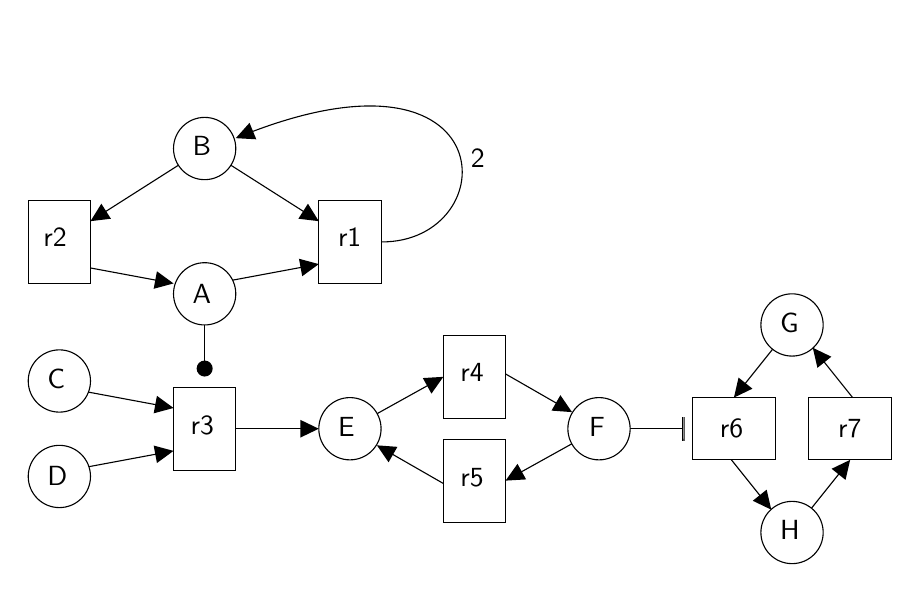
\begin{tikzpicture}[x=0.75pt,y=0.75pt,yscale=-1,xscale=1]
%uncomment if require: \path (0,300); %set diagram left start at 0, and has height of 300

%Straight Lines [id:da3576438741903769] 
\draw    (388,210) -- (414.13,177.34) ;
\draw [shift={(416,175)}, rotate = 488.66] [fill={rgb, 255:red, 0; green, 0; blue, 0 }  ][line width=0.08]  [draw opacity=0] (8.93,-4.29) -- (0,0) -- (8.93,4.29) -- cycle    ;
%Straight Lines [id:da5206527388854192] 
\draw    (350,164) -- (376.13,196.66) ;
\draw [shift={(378,199)}, rotate = 231.34] [fill={rgb, 255:red, 0; green, 0; blue, 0 }  ][line width=0.08]  [draw opacity=0] (8.93,-4.29) -- (0,0) -- (8.93,4.29) -- cycle    ;
%Straight Lines [id:da9664135693242828] 
\draw    (388,110) -- (361.87,142.66) ;
\draw [shift={(360,145)}, rotate = 308.65999999999997] [fill={rgb, 255:red, 0; green, 0; blue, 0 }  ][line width=0.08]  [draw opacity=0] (8.93,-4.29) -- (0,0) -- (8.93,4.29) -- cycle    ;
%Straight Lines [id:da3150124855239005] 
\draw    (426,156) -- (399.87,123.34) ;
\draw [shift={(398,121)}, rotate = 411.34000000000003] [fill={rgb, 255:red, 0; green, 0; blue, 0 }  ][line width=0.08]  [draw opacity=0] (8.93,-4.29) -- (0,0) -- (8.93,4.29) -- cycle    ;
%Straight Lines [id:da2531638133399581] 
\draw    (295,160) -- (335,160) ;
%Straight Lines [id:da7978054588524539] 
\draw    (110,160) -- (157,160) ;
\draw [shift={(160,160)}, rotate = 180] [fill={rgb, 255:red, 0; green, 0; blue, 0 }  ][line width=0.08]  [draw opacity=0] (8.93,-4.29) -- (0,0) -- (8.93,4.29) -- cycle    ;
%Straight Lines [id:da5621074466789615] 
\draw    (235,125) -- (279.4,150.51) ;
\draw [shift={(282,152)}, rotate = 209.88] [fill={rgb, 255:red, 0; green, 0; blue, 0 }  ][line width=0.08]  [draw opacity=0] (8.93,-4.29) -- (0,0) -- (8.93,4.29) -- cycle    ;
%Straight Lines [id:da9432384230142636] 
\draw    (235,195) -- (190.6,169.49) ;
\draw [shift={(188,168)}, rotate = 389.88] [fill={rgb, 255:red, 0; green, 0; blue, 0 }  ][line width=0.08]  [draw opacity=0] (8.93,-4.29) -- (0,0) -- (8.93,4.29) -- cycle    ;
%Straight Lines [id:da2732887752012232] 
\draw    (295,160) -- (252.62,183.54) ;
\draw [shift={(250,185)}, rotate = 330.95] [fill={rgb, 255:red, 0; green, 0; blue, 0 }  ][line width=0.08]  [draw opacity=0] (8.93,-4.29) -- (0,0) -- (8.93,4.29) -- cycle    ;
%Straight Lines [id:da8361705783456022] 
\draw    (175,160) -- (217.38,136.46) ;
\draw [shift={(220,135)}, rotate = 510.95] [fill={rgb, 255:red, 0; green, 0; blue, 0 }  ][line width=0.08]  [draw opacity=0] (8.93,-4.29) -- (0,0) -- (8.93,4.29) -- cycle    ;
%Straight Lines [id:da26704871020062715] 
\draw    (110,90) -- (157.05,81.23) ;
\draw [shift={(160,80.68)}, rotate = 529.44] [fill={rgb, 255:red, 0; green, 0; blue, 0 }  ][line width=0.08]  [draw opacity=0] (8.93,-4.29) -- (0,0) -- (8.93,4.29) -- cycle    ;
%Straight Lines [id:da4846937260313433] 
\draw    (40,80.68) -- (87.05,89.45) ;
\draw [shift={(90,90)}, rotate = 190.56] [fill={rgb, 255:red, 0; green, 0; blue, 0 }  ][line width=0.08]  [draw opacity=0] (8.93,-4.29) -- (0,0) -- (8.93,4.29) -- cycle    ;
%Straight Lines [id:da271105016276878] 
\draw    (105,25) -- (157.47,58.39) ;
\draw [shift={(160,60)}, rotate = 212.47] [fill={rgb, 255:red, 0; green, 0; blue, 0 }  ][line width=0.08]  [draw opacity=0] (8.93,-4.29) -- (0,0) -- (8.93,4.29) -- cycle    ;
%Shape: Rectangle [id:dp9228181661849988] 
\draw  [fill={rgb, 255:red, 255; green, 255; blue, 255 }  ,fill opacity=1 ] (20,50) -- (50,50) -- (50,90) -- (20,90) -- cycle ;
%Straight Lines [id:da06467494297119436] 
\draw    (105,25) -- (52.53,58.39) ;
\draw [shift={(50,60)}, rotate = 327.53] [fill={rgb, 255:red, 0; green, 0; blue, 0 }  ][line width=0.08]  [draw opacity=0] (8.93,-4.29) -- (0,0) -- (8.93,4.29) -- cycle    ;
%Shape: Circle [id:dp49236484975772] 
\draw  [fill={rgb, 255:red, 255; green, 255; blue, 255 }  ,fill opacity=1 ] (90,25) .. controls (90,16.72) and (96.72,10) .. (105,10) .. controls (113.28,10) and (120,16.72) .. (120,25) .. controls (120,33.28) and (113.28,40) .. (105,40) .. controls (96.72,40) and (90,33.28) .. (90,25) -- cycle ;
%Shape: Rectangle [id:dp3146550401206405] 
\draw  [fill={rgb, 255:red, 255; green, 255; blue, 255 }  ,fill opacity=1 ] (160,50) -- (190,50) -- (190,90) -- (160,90) -- cycle ;
%Curve Lines [id:da9984566963389516] 
\draw    (190,70) .. controls (250.06,70.4) and (250.75,-32.96) .. (121.95,19.2) ;
\draw [shift={(120,20)}, rotate = 337.56] [fill={rgb, 255:red, 0; green, 0; blue, 0 }  ][line width=0.08]  [draw opacity=0] (8.93,-4.29) -- (0,0) -- (8.93,4.29) -- cycle    ;
%Shape: Circle [id:dp09345090103745823] 
\draw  [fill={rgb, 255:red, 255; green, 255; blue, 255 }  ,fill opacity=1 ] (90,95) .. controls (90,86.72) and (96.72,80) .. (105,80) .. controls (113.28,80) and (120,86.72) .. (120,95) .. controls (120,103.28) and (113.28,110) .. (105,110) .. controls (96.72,110) and (90,103.28) .. (90,95) -- cycle ;
%Straight Lines [id:da5223576478149881] 
\draw    (105,110) -- (105,131) ;
\draw [shift={(105,131)}, rotate = 90] [color={rgb, 255:red, 0; green, 0; blue, 0 }  ][fill={rgb, 255:red, 0; green, 0; blue, 0 }  ][line width=0.75]      (0, 0) circle [x radius= 3.35, y radius= 3.35]   ;
%Shape: Rectangle [id:dp25364205729175127] 
\draw  [fill={rgb, 255:red, 255; green, 255; blue, 255 }  ,fill opacity=1 ] (90,140) -- (120,140) -- (120,180) -- (90,180) -- cycle ;
%Straight Lines [id:da8084682726089965] 
\draw    (40,140.68) -- (87.05,149.45) ;
\draw [shift={(90,150)}, rotate = 190.56] [fill={rgb, 255:red, 0; green, 0; blue, 0 }  ][line width=0.08]  [draw opacity=0] (8.93,-4.29) -- (0,0) -- (8.93,4.29) -- cycle    ;
%Straight Lines [id:da8278541197200837] 
\draw    (40,180) -- (87.05,171.23) ;
\draw [shift={(90,170.68)}, rotate = 529.44] [fill={rgb, 255:red, 0; green, 0; blue, 0 }  ][line width=0.08]  [draw opacity=0] (8.93,-4.29) -- (0,0) -- (8.93,4.29) -- cycle    ;
%Shape: Circle [id:dp5697702501712039] 
\draw  [fill={rgb, 255:red, 255; green, 255; blue, 255 }  ,fill opacity=1 ] (20,137) .. controls (20,128.72) and (26.72,122) .. (35,122) .. controls (43.28,122) and (50,128.72) .. (50,137) .. controls (50,145.28) and (43.28,152) .. (35,152) .. controls (26.72,152) and (20,145.28) .. (20,137) -- cycle ;
%Shape: Circle [id:dp027027959729662543] 
\draw  [fill={rgb, 255:red, 255; green, 255; blue, 255 }  ,fill opacity=1 ] (20,183) .. controls (20,174.72) and (26.72,168) .. (35,168) .. controls (43.28,168) and (50,174.72) .. (50,183) .. controls (50,191.28) and (43.28,198) .. (35,198) .. controls (26.72,198) and (20,191.28) .. (20,183) -- cycle ;
%Shape: Circle [id:dp7929646959402241] 
\draw  [fill={rgb, 255:red, 255; green, 255; blue, 255 }  ,fill opacity=1 ] (160,160) .. controls (160,151.72) and (166.72,145) .. (175,145) .. controls (183.28,145) and (190,151.72) .. (190,160) .. controls (190,168.28) and (183.28,175) .. (175,175) .. controls (166.72,175) and (160,168.28) .. (160,160) -- cycle ;
%Shape: Rectangle [id:dp05655391624383377] 
\draw  [fill={rgb, 255:red, 255; green, 255; blue, 255 }  ,fill opacity=1 ] (220,115) -- (250,115) -- (250,155) -- (220,155) -- cycle ;
%Shape: Rectangle [id:dp05796590340987029] 
\draw  [fill={rgb, 255:red, 255; green, 255; blue, 255 }  ,fill opacity=1 ] (220,165) -- (250,165) -- (250,205) -- (220,205) -- cycle ;
%Shape: Circle [id:dp13273124949760895] 
\draw  [fill={rgb, 255:red, 255; green, 255; blue, 255 }  ,fill opacity=1 ] (280,160) .. controls (280,151.72) and (286.72,145) .. (295,145) .. controls (303.28,145) and (310,151.72) .. (310,160) .. controls (310,168.28) and (303.28,175) .. (295,175) .. controls (286.72,175) and (280,168.28) .. (280,160) -- cycle ;
%Straight Lines [id:da9347007050049654] 
\draw    (335.29,154.43) -- (335.26,165.81) ;
%Straight Lines [id:da20553639689795267] 
\draw    (336,154.43) -- (335.97,165.81) ;
%Shape: Rectangle [id:dp30165349356224813] 
\draw  [fill={rgb, 255:red, 255; green, 255; blue, 255 }  ,fill opacity=1 ] (380,145) -- (380,175) -- (340,175) -- (340,145) -- cycle ;
%Shape: Rectangle [id:dp05448702121100979] 
\draw  [fill={rgb, 255:red, 255; green, 255; blue, 255 }  ,fill opacity=1 ] (436,145) -- (436,175) -- (396,175) -- (396,145) -- cycle ;
%Shape: Circle [id:dp37659499504730287] 
\draw  [fill={rgb, 255:red, 255; green, 255; blue, 255 }  ,fill opacity=1 ] (373,110) .. controls (373,101.72) and (379.72,95) .. (388,95) .. controls (396.28,95) and (403,101.72) .. (403,110) .. controls (403,118.28) and (396.28,125) .. (388,125) .. controls (379.72,125) and (373,118.28) .. (373,110) -- cycle ;
%Shape: Circle [id:dp13055596917815526] 
\draw  [fill={rgb, 255:red, 255; green, 255; blue, 255 }  ,fill opacity=1 ] (373,210) .. controls (373,201.72) and (379.72,195) .. (388,195) .. controls (396.28,195) and (403,201.72) .. (403,210) .. controls (403,218.28) and (396.28,225) .. (388,225) .. controls (379.72,225) and (373,218.28) .. (373,210) -- cycle ;

% Text Node
\draw (26,62) node [anchor=north west][inner sep=0.75pt]   [align=left] {$\mathsf{r2}$};
% Text Node
\draw (168,62) node [anchor=north west][inner sep=0.75pt]   [align=left] {$\mathsf{r1}$};
% Text Node
\draw (97,153) node [anchor=north west][inner sep=0.75pt]   [align=left] {$\mathsf{r3}$};
% Text Node
\draw (227,127) node [anchor=north west][inner sep=0.75pt]   [align=left] {$\mathsf{r4}$};
% Text Node
\draw (227,178) node [anchor=north west][inner sep=0.75pt]   [align=left] {$\mathsf{r5}$};
% Text Node
\draw (352,154) node [anchor=north west][inner sep=0.75pt]   [align=left] {$\mathsf{r6}$};
% Text Node
\draw (409,154) node [anchor=north west][inner sep=0.75pt]   [align=left] {$\mathsf{r7}$};

% Text Node
\draw (98,18) node [anchor=north west][inner sep=0.75pt]   [align=left] {$\mathsf{B}$};
% Text Node
\draw (98,89) node [anchor=north west][inner sep=0.75pt]   [align=left] {$\mathsf{A}$};
% Text Node
\draw (28,130) node [anchor=north west][inner sep=0.75pt]   [align=left] {$\mathsf{C}$};
% Text Node
\draw (28,177) node [anchor=north west][inner sep=0.75pt]   [align=left] {$\mathsf{D}$};
% Text Node
\draw (168,153) node [anchor=north west][inner sep=0.75pt]   [align=left] {$\mathsf{E}$};
% Text Node
\draw (289,153) node [anchor=north west][inner sep=0.75pt]   [align=left] {$\mathsf{F}$};
% Text Node
\draw (381,103) node [anchor=north west][inner sep=0.75pt]   [align=left] {$\mathsf{G}$};
% Text Node
\draw (381,203) node [anchor=north west][inner sep=0.75pt]   [align=left] {$\mathsf{H}$};
% Text Node
\draw (232,24) node [anchor=north west][inner sep=0.75pt]   [align=left] {$\mathsf{2}$};


\end{tikzpicture}}
    \caption{The Pathway Petri Net corresponding to the reactions described in Figure \ref{subfig:example-reactions}}
    \label{subfig:pathway-petri-net}
\end{figure*}

In this work, we use a variant of \glspl{ppn} where all the information unrelated to the structure of the pathway is discarded. Specifically, we ignore information about:
\begin{itemize}
    \item kinetic formulas;
    \item multiplicities of reactants and products (\ie edge labels);
    \item the initial marking $M_0$.
\end{itemize}
Basically, for our purposes, a \gls{ppn} is a tuple $\wp = \Tuple{\Cal{P},\Cal{T},\Cal{A}_{S}, \Cal{A}_{P},\Cal{A}_{I}}$ where the irrelevant components have been omitted. We rewrite this object, according to the graph notation introduced in Section \ref{sec:graphs}, into a \keyword{pathway graph} $G = \Tuple{\Cal{V}_G, \Cal{E}_G}$. To do so, we first define the following nodes and edges subsets:
\begin{itemize}
    \item $\Cal{V}_{G}^{\Fun{mol}} = \Cal{P}$ is the set of molecules;
    \item $\Cal{V}_{G}^{\Fun{rx}} = \Cal{T}$ is the set of reactions;
    \item $\Cal{E}_{G}^{\Fun{std}} = \Cal{A}_S$ is the set of standard edges;
    \item $\Cal{E}_{G}^{\Fun{pro}} = \Cal{A}_P$ is the set of promoter edges;
    \item $\Cal{E}_{G}^{\Fun{inh}} = \Cal{A}_I$ is the set of inhibitor edges,
\end{itemize}
where $\Cal{V}_{G}^{\Fun{mol}} \Inter \Cal{V}_{G}^{\Fun{rx}} = \emptyset$ and $\Cal{E}_{G}^{\Fun{std}} \Inter \Cal{E}_{G}^{\Fun{pro}} \Inter \Cal{E}_{G}^{\Fun{inh}} = \emptyset$. Then, we simply set $\Cal{V}_G = \Cal{V}_G^{\Fun{mol}} \Union \Cal{V}_G^{\Fun{rx}}$ and $\Cal{E}_G = \Cal{E}_G^{\Fun{std}} \Union \Cal{E}_G^{\Fun{pro}} \Union \Cal{E}_G^{\Fun{inh}}$.
Using the biochemical pathway of Figure \ref{fig:example-pathway} as reference, its associated pathway graph is shown in Figure \ref{fig:pathway-graph}.
\begin{figure*}[h!]
    \centering
    \resizebox{.6\textwidth}{!}{

\tikzset{every picture/.style={line width=0.75pt}} %set default line width to 0.75pt

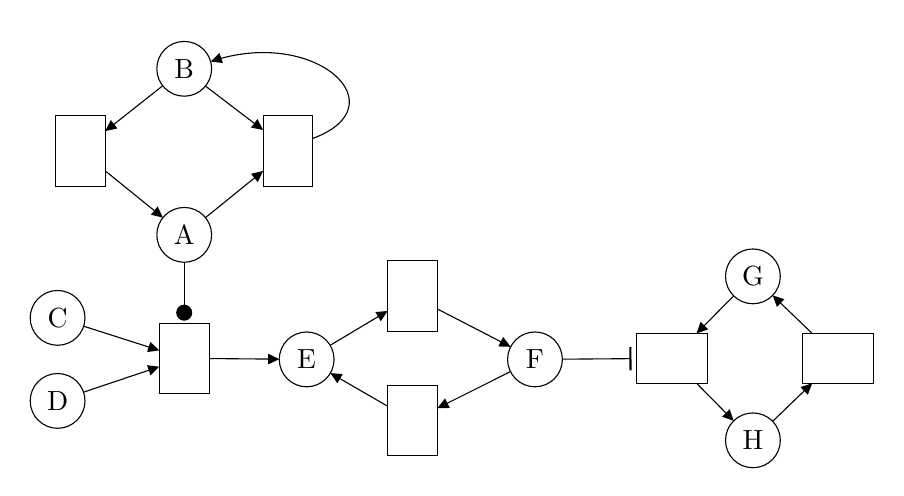
\begin{tikzpicture}[x=0.75pt,y=0.75pt,yscale=-1,xscale=1]
%uncomment if require: \path (0,300); %set diagram left start at 0, and has height of 300

%Straight Lines [id:da289255485986883]
\draw    (100,56) -- (135.62,83.18) ;
\draw [shift={(138,85)}, rotate = 217.35] [fill={rgb, 255:red, 0; green, 0; blue, 0 }  ][line width=0.08]  [draw opacity=0] (5.36,-2.57) -- (0,0) -- (5.36,2.57) -- cycle    ;

% Text Node
\draw  [fill={rgb, 255:red, 255; green, 255; blue, 255 }  ,fill opacity=1 ]  (38,78) -- (62,78) -- (62,112) -- (38,112) -- cycle  ;
\draw (50,95) node   [align=left] {\begin{minipage}[lt]{13.600000000000001pt}\setlength\topsep{0pt}
\begin{center}
\end{center}

\end{minipage}};
% Text Node
\draw  [fill={rgb, 255:red, 255; green, 255; blue, 255 }  ,fill opacity=1 ]  (100, 55.5) circle [x radius= 13.2, y radius= 13.2]   ;
\draw (100,55.5) node   [align=left] {\begin{minipage}[lt]{14.96pt}\setlength\topsep{0pt}
\begin{center}
\SF{B}
\end{center}

\end{minipage}};
% Text Node
\draw  [fill={rgb, 255:red, 255; green, 255; blue, 255 }  ,fill opacity=1 ]  (138,78) -- (162,78) -- (162,112) -- (138,112) -- cycle  ;
\draw (150,95) node   [align=left] {\begin{minipage}[lt]{13.600000000000001pt}\setlength\topsep{0pt}
\begin{center}
\end{center}

\end{minipage}};
% Text Node
\draw  [fill={rgb, 255:red, 255; green, 255; blue, 255 }  ,fill opacity=1 ]  (100, 135.5) circle [x radius= 13.2, y radius= 13.2]   ;
\draw (100,135.5) node   [align=left] {\begin{minipage}[lt]{14.96pt}\setlength\topsep{0pt}
\begin{center}
\SF{A}
\end{center}

\end{minipage}};
% Text Node
\draw  [fill={rgb, 255:red, 255; green, 255; blue, 255 }  ,fill opacity=1 ]  (39, 175.5) circle [x radius= 13.2, y radius= 13.2]   ;
\draw (39,175.5) node   [align=left] {\begin{minipage}[lt]{14.96pt}\setlength\topsep{0pt}
\begin{center}
\SF{C}
\end{center}

\end{minipage}};
% Text Node
\draw  [fill={rgb, 255:red, 255; green, 255; blue, 255 }  ,fill opacity=1 ]  (39, 215.5) circle [x radius= 13.2, y radius= 13.2]   ;
\draw (39,215.5) node   [align=left] {\begin{minipage}[lt]{14.96pt}\setlength\topsep{0pt}
\begin{center}
\SF{D}
\end{center}

\end{minipage}};
% Text Node
\draw  [fill={rgb, 255:red, 255; green, 255; blue, 255 }  ,fill opacity=1 ]  (88,178) -- (112,178) -- (112,212) -- (88,212) -- cycle  ;
\draw (100,195) node   [align=left] {\begin{minipage}[lt]{13.600000000000001pt}\setlength\topsep{0pt}
\begin{center}
\end{center}

\end{minipage}};
% Text Node
\draw  [fill={rgb, 255:red, 255; green, 255; blue, 255 }  ,fill opacity=1 ]  (159, 195.5) circle [x radius= 13.2, y radius= 13.2]   ;
\draw (159,195.5) node   [align=left] {\begin{minipage}[lt]{14.96pt}\setlength\topsep{0pt}
\begin{center}
\SF{E}
\end{center}

\end{minipage}};
% Text Node
\draw  [fill={rgb, 255:red, 255; green, 255; blue, 255 }  ,fill opacity=1 ]  (198,148) -- (222,148) -- (222,182) -- (198,182) -- cycle  ;
\draw (210,165) node   [align=left] {\begin{minipage}[lt]{13.600000000000001pt}\setlength\topsep{0pt}
\begin{center}
\end{center}

\end{minipage}};
% Text Node
\draw  [fill={rgb, 255:red, 255; green, 255; blue, 255 }  ,fill opacity=1 ]  (198,208) -- (222,208) -- (222,242) -- (198,242) -- cycle  ;
\draw (210,225) node   [align=left] {\begin{minipage}[lt]{13.600000000000001pt}\setlength\topsep{0pt}
\begin{center}
\end{center}

\end{minipage}};
% Text Node
\draw  [fill={rgb, 255:red, 255; green, 255; blue, 255 }  ,fill opacity=1 ]  (269, 195.5) circle [x radius= 13.2, y radius= 13.2]   ;
\draw (269,195.5) node   [align=left] {\begin{minipage}[lt]{14.96pt}\setlength\topsep{0pt}
\begin{center}
\SF{F}
\end{center}

\end{minipage}};
% Text Node
\draw  [fill={rgb, 255:red, 255; green, 255; blue, 255 }  ,fill opacity=1 ]  (318,183) -- (352,183) -- (352,207) -- (318,207) -- cycle  ;
\draw (335,195) node   [align=left] {\begin{minipage}[lt]{20.400000000000002pt}\setlength\topsep{0pt}
\begin{center}
\end{center}

\end{minipage}};
% Text Node
\draw  [fill={rgb, 255:red, 255; green, 255; blue, 255 }  ,fill opacity=1 ]  (398,183) -- (432,183) -- (432,207) -- (398,207) -- cycle  ;
\draw (415,195) node   [align=left] {\begin{minipage}[lt]{20.400000000000002pt}\setlength\topsep{0pt}
\begin{center}
\end{center}

\end{minipage}};
% Text Node
\draw  [fill={rgb, 255:red, 255; green, 255; blue, 255 }  ,fill opacity=1 ]  (374, 155.5) circle [x radius= 13.2, y radius= 13.2]   ;
\draw (374,155.5) node   [align=left] {\begin{minipage}[lt]{14.96pt}\setlength\topsep{0pt}
\begin{center}
\SF{G}
\end{center}

\end{minipage}};
% Text Node
\draw  [fill={rgb, 255:red, 255; green, 255; blue, 255 }  ,fill opacity=1 ]  (374, 234.5) circle [x radius= 13.2, y radius= 13.2]   ;
\draw (374,234.5) node   [align=left] {\begin{minipage}[lt]{14.96pt}\setlength\topsep{0pt}
\begin{center}
\SF{H}
\end{center}

\end{minipage}};
% Connection
\draw    (89.64,63.68) -- (64.35,83.66) ;
\draw [shift={(62,85.52)}, rotate = 321.69] [fill={rgb, 255:red, 0; green, 0; blue, 0 }  ][line width=0.08]  [draw opacity=0] (5.36,-2.57) -- (0,0) -- (5.36,2.57) -- cycle    ;
% Connection
\draw    (62,104.72) -- (87.41,125.3) ;
\draw [shift={(89.74,127.19)}, rotate = 219.01] [fill={rgb, 255:red, 0; green, 0; blue, 0 }  ][line width=0.08]  [draw opacity=0] (5.36,-2.57) -- (0,0) -- (5.36,2.57) -- cycle    ;
% Connection
\draw    (110.26,127.19) -- (135.67,106.61) ;
\draw [shift={(138,104.72)}, rotate = 500.99] [fill={rgb, 255:red, 0; green, 0; blue, 0 }  ][line width=0.08]  [draw opacity=0] (5.36,-2.57) -- (0,0) -- (5.36,2.57) -- cycle    ;
% Connection
\draw    (100,148.7) -- (100,173) ;
\draw [shift={(100,173)}, rotate = 90] [color={rgb, 255:red, 0; green, 0; blue, 0 }  ][fill={rgb, 255:red, 0; green, 0; blue, 0 }  ][line width=0.75]      (0, 0) circle [x radius= 3.35, y radius= 3.35]   ;
% Connection
\draw    (162,89.03) .. controls (203.8,73.44) and (164.07,35.95) .. (114.99,51.28) ;
\draw [shift={(112.74,52.02)}, rotate = 341.03] [fill={rgb, 255:red, 0; green, 0; blue, 0 }  ][line width=0.08]  [draw opacity=0] (5.36,-2.57) -- (0,0) -- (5.36,2.57) -- cycle    ;
% Connection
\draw    (51.58,179.52) -- (85.14,190.25) ;
\draw [shift={(88,191.16)}, rotate = 197.73] [fill={rgb, 255:red, 0; green, 0; blue, 0 }  ][line width=0.08]  [draw opacity=0] (5.36,-2.57) -- (0,0) -- (5.36,2.57) -- cycle    ;
% Connection
\draw    (51.52,211.29) -- (85.16,199.99) ;
\draw [shift={(88,199.03)}, rotate = 521.4200000000001] [fill={rgb, 255:red, 0; green, 0; blue, 0 }  ][line width=0.08]  [draw opacity=0] (5.36,-2.57) -- (0,0) -- (5.36,2.57) -- cycle    ;
% Connection
\draw    (112,195.1) -- (142.8,195.36) ;
\draw [shift={(145.8,195.39)}, rotate = 180.49] [fill={rgb, 255:red, 0; green, 0; blue, 0 }  ][line width=0.08]  [draw opacity=0] (5.36,-2.57) -- (0,0) -- (5.36,2.57) -- cycle    ;
% Connection
\draw    (170.33,188.72) -- (195.43,173.72) ;
\draw [shift={(198,172.18)}, rotate = 509.12] [fill={rgb, 255:red, 0; green, 0; blue, 0 }  ][line width=0.08]  [draw opacity=0] (5.36,-2.57) -- (0,0) -- (5.36,2.57) -- cycle    ;
% Connection
\draw    (222,171.2) -- (254.61,188.06) ;
\draw [shift={(257.27,189.44)}, rotate = 207.34] [fill={rgb, 255:red, 0; green, 0; blue, 0 }  ][line width=0.08]  [draw opacity=0] (5.36,-2.57) -- (0,0) -- (5.36,2.57) -- cycle    ;
% Connection
\draw    (257.19,201.4) -- (224.68,217.66) ;
\draw [shift={(222,219)}, rotate = 333.43] [fill={rgb, 255:red, 0; green, 0; blue, 0 }  ][line width=0.08]  [draw opacity=0] (5.36,-2.57) -- (0,0) -- (5.36,2.57) -- cycle    ;
% Connection
\draw    (198,218.06) -- (173.03,203.61) ;
\draw [shift={(170.43,202.11)}, rotate = 390.05] [fill={rgb, 255:red, 0; green, 0; blue, 0 }  ][line width=0.08]  [draw opacity=0] (5.36,-2.57) -- (0,0) -- (5.36,2.57) -- cycle    ;
% Connection
\draw    (282.2,195.4) -- (315,195.15) ;
\draw [shift={(315,195.15)}, rotate = 539.5699999999999] [color={rgb, 255:red, 0; green, 0; blue, 0 }  ][line width=0.75]    (0,5.59) -- (0,-5.59)   ;
% Connection
\draw    (346.85,207) -- (362.62,222.97) ;
\draw [shift={(364.73,225.11)}, rotate = 225.36] [fill={rgb, 255:red, 0; green, 0; blue, 0 }  ][line width=0.08]  [draw opacity=0] (5.36,-2.57) -- (0,0) -- (5.36,2.57) -- cycle    ;
% Connection
\draw    (383.51,225.34) -- (400.38,209.08) ;
\draw [shift={(402.54,207)}, rotate = 496.07] [fill={rgb, 255:red, 0; green, 0; blue, 0 }  ][line width=0.08]  [draw opacity=0] (5.36,-2.57) -- (0,0) -- (5.36,2.57) -- cycle    ;
% Connection
\draw    (402.54,183) -- (385.67,166.74) ;
\draw [shift={(383.51,164.66)}, rotate = 403.93] [fill={rgb, 255:red, 0; green, 0; blue, 0 }  ][line width=0.08]  [draw opacity=0] (5.36,-2.57) -- (0,0) -- (5.36,2.57) -- cycle    ;
% Connection
\draw    (364.73,164.89) -- (348.96,180.87) ;
\draw [shift={(346.85,183)}, rotate = 314.64] [fill={rgb, 255:red, 0; green, 0; blue, 0 }  ][line width=0.08]  [draw opacity=0] (5.36,-2.57) -- (0,0) -- (5.36,2.57) -- cycle    ;

\end{tikzpicture}}
    \caption{The pathway graph obtained by omitting kinetic formulas and edge labels from the one in Figure \ref{subfig:pathway-petri-net}. Notice that the names of the molecules are displayed for visual aid, but are not included of the pathway graph.}
    \label{fig:pathway-graph}
\end{figure*}
More explicitly, the set of nodes of the pathway graph contains both molecules and reactions. The set of edges of the graph contains an edge (of any type) from a molecule to a reaction if and only if a perturbation in the concentration of the molecule determines a change in the reaction rate (that could in principle be computed through the omitted kinetic formula). Similarly, it contains an edge from a reaction to a molecule if and only if a perturbation in the reaction rate determines a change in the dynamics of the concentration of that molecule. This is intuitive for those molecular species that are products, as the dynamics of the product accumulation is determined by the reaction rate. By construction, a pathway graph is bipartite.

\subsection{Concentration Robustness}\label{sect:robustness}
Robustness is defined as the ability of a system to maintain its functionalities again external and internal perturbations \cite{?}, a property observed in many biological systems. A general notion of robustness has been formalized by Kitano in \cite{?}. This formalization considers a specific functionality of a system and the \emph{viability} of such functionality, defined as the ability of the system (\eg a cell) to carry it out. This could be expressed, for instance, in terms of the synthesis/degradation rate or concentration level of some target substance, in terms of cell growth rate, or in terms of  other suitable quantitative indicators. More specifically, according to Kitano's definition, the robustness $R$ of a system $\mathbb{S}$, with respect to a specific functionality $a$ and against a set of perturbations $P$ is expressed as:
\[
 R^{\mathbb{S}}_{a,P} = \int_p \Psi(p) D_a^\mathbb{S}(p)dp
\]
In the above definition, $\Psi(p)$ is the probability a perturbation $p$, and $D_a(p)$ evaluates the functionality $a$ of the system $\mathbb{S}$ under the perturbation $p$. More precisely, function $D_a(p)$ gives the viability of $a$ under perturbation $p$, in relation to the viability of $a$ under normal conditions. In the absence of perturbations, $D_a(p)=1$, meaning that the functionality $a$ is assumed to be carried out in an optimal way, or equivalently, that perturbations have irrelevant or no influence; conversely, $D_a(p) = 0$ if perturbations cause the system to fail completely in performing $a$, and $0 < D_a(p) < 1$ in the case of relevant perturbations.
    
An improvement to Kitano's formulation of robustness has been proposed in \cite{?}, where functionalities to be maintained are described as linear temporal logic (LTL) formulas. In this formulation, the impact of perturbations is quantified through a notion of \emph{violation degree}, which measures the distance between the dynamics of the perturbed system and the LTL formula. Many more specific definitions exist, differing either in the class of biological systems they apply to, or in the way the functionality to be maintained is expressed \cite{?}. 

In the case of biochemical pathways, a common formulation of robustness can be expressed in terms of maintenance of the concentration levels of some species. This definition can be reduced to both general formulations in \cite{?} and \cite{?}. In particular, the \emph{absolute concentration robustness} proposed in \cite{?} is based on the comparison of the concentration level of given species at the steady state, against perturbations (either in the kinetic parameters or in the initial concentrations) of some other species.

A generalization of absolute concentration robustness, called \emph{$\alpha$-robustness}, has been proposed in \cite{?}, where concentration intervals are introduced both for the perturbed molecules (input species) and for the molecules whose concentration is maintained (output species). Informally speaking, a biochemical pathway is $\alpha$-robust with respect to a given set of initial concentration intervals, if the concentration of a chosen output molecule at the steady state lies in the interval $[k-\alpha/2,k+\alpha/2]$ for some $k \in \mathbb{R}$. A relative version of $\alpha$-robustness can be obtained simply by dividing $\alpha$ by $k$. This notion of $\alpha$-robustness is related to the notion of global sensitivity \cite{?}, which typically measures the average effect of a set of perturbations. Hereafter, we use the term robustness to specifically refer to \emph{$\alpha$-robustness} for brevity.

The assessment of robustness usually requires to perform exhaustive numerical simulations in parameter space \cite{?,?} (where by parameters we intend mainly the kinetic parameters, or the initial concentrations). In some particular cases, one can exploit the biological network structure to avoid performing simulations altogether \cite{?}. Moreover, in cases where the dynamics of the network are monotonic, the number of such simulations can be significantly reduced \cite{?}.

\section{Methods}
Our framework to process the biochemical pathways consists of a \gls{dgn} which takes a pathway and a pair of input/output nodes on which the robustness is defined, and predicts whether this structure is robust or not with a downstream classifier. Here, we describe the methodology used to transform the raw biochemical pathways into a dataset of graphs used to train our model to predict robustness.

\subsection{Data Collection}\label{subsec:data-collection}
Our initial dataset is composed of 706 SBML models of biochemical pathways, downloaded from the BioModels database \cite{?}. Specifically, the data correspond to the complete set of manually curated models present in the database at the time we started the construction of the dataset\footnote{May 2019.}. We removed empty models (not containing any node) and discarded duplicates, reducing the number of SBML models to 484. These models, were first transformed into \glspl{ppn} representations, which were saved in DOT format\footnote{The DOT graph description language specification, available at: \url{https://graphviz.gitlab.io/_pages/doc/info/lang.html}}. For the translation of the SMBL models into \glspl{ppn}, we developed a Python script that, for each reaction in the SMBL model extracts reactants, products and modifiers. Furthermore, it also checks the kinetic formula in order to determine whether each modifier is either promoter or an inhibitor. Each \gls{ppn} has been finally converted into a pathway graph, resulting in a set $\mathbb{G}$ defined as: $$\mathbb{G} = \Set{G_{i}}_{i=1}^{484},$$
where $G_i$ is the pathway graph of the $i$-th \gls{ppn}.

\subsection{Dataset Construction}
After obtaining the set of pathway graphs as described above, we proceeded to derive the of training subgraphs to which a robustness value is associated. Before delving into details, let us first introduce a helper data structure which we call \keyword{enriched pathway graph}. Given a pathway graph $G$, its enriched version $G'$ is defined as follows: initially, $\Cal{V}_{G'}=\Cal{V}_G$, $\Cal{E}_{G'}=\Cal{E}_G$. Then, for every standard edge $(u, v) \in \Cal{E}_{G}^{\Fun{std}}$ where $u \in \Cal{V}_{G}^{\Fun{mol}}$ and $v \in \Cal{E}_{G}^{\Fun{rx}}$, we update the standard edges of $G'$ with a reverse standard edge $(v,u)$, setting $\Cal{E}_{G'}^{\Fun{std}} = \Cal{E}_{G'}^{\Fun{std}} \Union (v, u)$. Note that we do not reverse neither standard edges from reactions to molecules, nor promotion and inhibition edges. The enriched pathway graph obtained from the pathway graph of Figure \ref{fig:pathway-graph} is shown in Figure \ref{fig:pathway-graph-enriched}, where the additional edges are drawn in solid black. Such graph represents influence relationships between molecules and reactions. The reversed edges encode the fact that a perturbation in the reaction rates determines a variation in the reactants consumption. Hence, the enriched pathway graph essentially corresponds to the \emph{influence graph} that could be computed from the Jacobian matrix containing the partial derivatives of the system of ODEs associated to the pathway \cite{?}.
\begin{figure*}[h!]
    \centering
    \resizebox{.6\textwidth}{!}{

\tikzset{every picture/.style={line width=0.75pt}} %set default line width to 0.75pt        

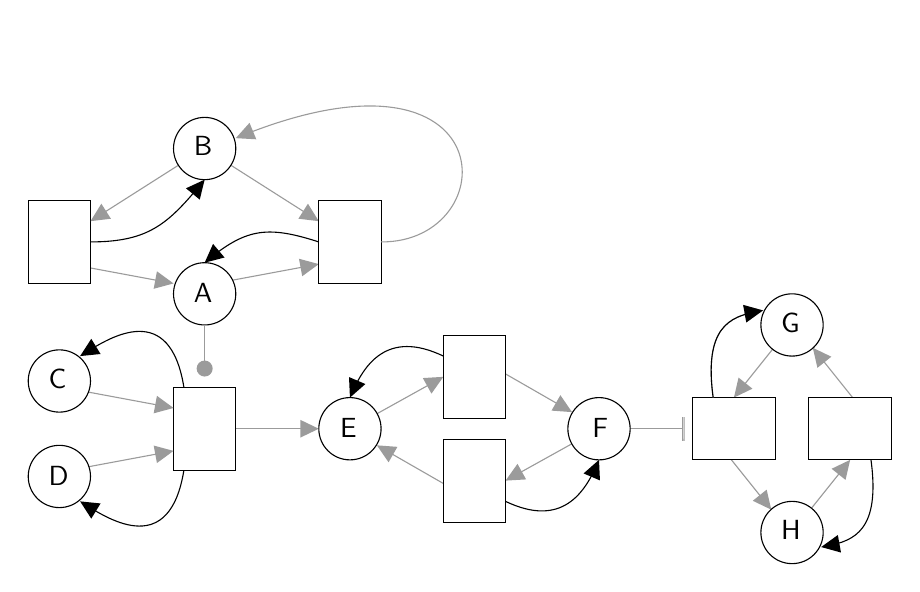
\begin{tikzpicture}[x=0.75pt,y=0.75pt,yscale=-1,xscale=1]
%uncomment if require: \path (0,300); %set diagram left start at 0, and has height of 300

%Straight Lines [id:da9814975397164354] 
\draw [color={rgb, 255:red, 155; green, 155; blue, 155 }  ,draw opacity=1 ]   (408,230) -- (434.13,197.34) ;
\draw [shift={(436,195)}, rotate = 488.66] [fill={rgb, 255:red, 155; green, 155; blue, 155 }  ,fill opacity=1 ][line width=0.08]  [draw opacity=0] (8.93,-4.29) -- (0,0) -- (8.93,4.29) -- cycle    ;
%Straight Lines [id:da9406459969344991] 
\draw [color={rgb, 255:red, 155; green, 155; blue, 155 }  ,draw opacity=1 ]   (370,184) -- (396.13,216.66) ;
\draw [shift={(398,219)}, rotate = 231.34] [fill={rgb, 255:red, 155; green, 155; blue, 155 }  ,fill opacity=1 ][line width=0.08]  [draw opacity=0] (8.93,-4.29) -- (0,0) -- (8.93,4.29) -- cycle    ;
%Straight Lines [id:da567762566187695] 
\draw [color={rgb, 255:red, 155; green, 155; blue, 155 }  ,draw opacity=1 ]   (408,130) -- (381.87,162.66) ;
\draw [shift={(380,165)}, rotate = 308.65999999999997] [fill={rgb, 255:red, 155; green, 155; blue, 155 }  ,fill opacity=1 ][line width=0.08]  [draw opacity=0] (8.93,-4.29) -- (0,0) -- (8.93,4.29) -- cycle    ;
%Straight Lines [id:da8407631771019597] 
\draw [color={rgb, 255:red, 155; green, 155; blue, 155 }  ,draw opacity=1 ]   (446,176) -- (419.87,143.34) ;
\draw [shift={(418,141)}, rotate = 411.34000000000003] [fill={rgb, 255:red, 155; green, 155; blue, 155 }  ,fill opacity=1 ][line width=0.08]  [draw opacity=0] (8.93,-4.29) -- (0,0) -- (8.93,4.29) -- cycle    ;
%Straight Lines [id:da18886988900572765] 
\draw [color={rgb, 255:red, 155; green, 155; blue, 155 }  ,draw opacity=1 ]   (315,180) -- (355,180) ;
%Straight Lines [id:da3931805508956303] 
\draw [color={rgb, 255:red, 155; green, 155; blue, 155 }  ,draw opacity=1 ]   (130,180) -- (177,180) ;
\draw [shift={(180,180)}, rotate = 180] [fill={rgb, 255:red, 155; green, 155; blue, 155 }  ,fill opacity=1 ][line width=0.08]  [draw opacity=0] (8.93,-4.29) -- (0,0) -- (8.93,4.29) -- cycle    ;
%Straight Lines [id:da8295871618343293] 
\draw [color={rgb, 255:red, 155; green, 155; blue, 155 }  ,draw opacity=1 ]   (255,145) -- (299.4,170.51) ;
\draw [shift={(302,172)}, rotate = 209.88] [fill={rgb, 255:red, 155; green, 155; blue, 155 }  ,fill opacity=1 ][line width=0.08]  [draw opacity=0] (8.93,-4.29) -- (0,0) -- (8.93,4.29) -- cycle    ;
%Straight Lines [id:da5331508184397238] 
\draw [color={rgb, 255:red, 155; green, 155; blue, 155 }  ,draw opacity=1 ]   (255,215) -- (210.6,189.49) ;
\draw [shift={(208,188)}, rotate = 389.88] [fill={rgb, 255:red, 155; green, 155; blue, 155 }  ,fill opacity=1 ][line width=0.08]  [draw opacity=0] (8.93,-4.29) -- (0,0) -- (8.93,4.29) -- cycle    ;
%Straight Lines [id:da9986006782985726] 
\draw [color={rgb, 255:red, 155; green, 155; blue, 155 }  ,draw opacity=1 ]   (315,180) -- (272.62,203.54) ;
\draw [shift={(270,205)}, rotate = 330.95] [fill={rgb, 255:red, 155; green, 155; blue, 155 }  ,fill opacity=1 ][line width=0.08]  [draw opacity=0] (8.93,-4.29) -- (0,0) -- (8.93,4.29) -- cycle    ;
%Straight Lines [id:da12348680583129257] 
\draw [color={rgb, 255:red, 155; green, 155; blue, 155 }  ,draw opacity=1 ]   (195,180) -- (237.38,156.46) ;
\draw [shift={(240,155)}, rotate = 510.95] [fill={rgb, 255:red, 155; green, 155; blue, 155 }  ,fill opacity=1 ][line width=0.08]  [draw opacity=0] (8.93,-4.29) -- (0,0) -- (8.93,4.29) -- cycle    ;
%Straight Lines [id:da9418451865861617] 
\draw [color={rgb, 255:red, 155; green, 155; blue, 155 }  ,draw opacity=1 ]   (130,110) -- (177.05,101.23) ;
\draw [shift={(180,100.68)}, rotate = 529.44] [fill={rgb, 255:red, 155; green, 155; blue, 155 }  ,fill opacity=1 ][line width=0.08]  [draw opacity=0] (8.93,-4.29) -- (0,0) -- (8.93,4.29) -- cycle    ;
%Straight Lines [id:da4404755375642728] 
\draw [color={rgb, 255:red, 155; green, 155; blue, 155 }  ,draw opacity=1 ]   (60,100.68) -- (107.05,109.45) ;
\draw [shift={(110,110)}, rotate = 190.56] [fill={rgb, 255:red, 155; green, 155; blue, 155 }  ,fill opacity=1 ][line width=0.08]  [draw opacity=0] (8.93,-4.29) -- (0,0) -- (8.93,4.29) -- cycle    ;
%Straight Lines [id:da30142710216357527] 
\draw [color={rgb, 255:red, 155; green, 155; blue, 155 }  ,draw opacity=1 ]   (125,45) -- (177.47,78.39) ;
\draw [shift={(180,80)}, rotate = 212.47] [fill={rgb, 255:red, 155; green, 155; blue, 155 }  ,fill opacity=1 ][line width=0.08]  [draw opacity=0] (8.93,-4.29) -- (0,0) -- (8.93,4.29) -- cycle    ;
%Shape: Rectangle [id:dp08787765148447635] 
\draw  [fill={rgb, 255:red, 255; green, 255; blue, 255 }  ,fill opacity=1 ] (40,70) -- (70,70) -- (70,110) -- (40,110) -- cycle ;
%Straight Lines [id:da003675026654497149] 
\draw [color={rgb, 255:red, 155; green, 155; blue, 155 }  ,draw opacity=1 ]   (125,45) -- (72.53,78.39) ;
\draw [shift={(70,80)}, rotate = 327.53] [fill={rgb, 255:red, 155; green, 155; blue, 155 }  ,fill opacity=1 ][line width=0.08]  [draw opacity=0] (8.93,-4.29) -- (0,0) -- (8.93,4.29) -- cycle    ;
%Shape: Circle [id:dp857493257636351] 
\draw  [fill={rgb, 255:red, 255; green, 255; blue, 255 }  ,fill opacity=1 ] (110,45) .. controls (110,36.72) and (116.72,30) .. (125,30) .. controls (133.28,30) and (140,36.72) .. (140,45) .. controls (140,53.28) and (133.28,60) .. (125,60) .. controls (116.72,60) and (110,53.28) .. (110,45) -- cycle ;
%Shape: Rectangle [id:dp06861100107998075] 
\draw  [fill={rgb, 255:red, 255; green, 255; blue, 255 }  ,fill opacity=1 ] (180,70) -- (210,70) -- (210,110) -- (180,110) -- cycle ;
%Curve Lines [id:da16899155142836797] 
\draw [color={rgb, 255:red, 155; green, 155; blue, 155 }  ,draw opacity=1 ]   (210,90) .. controls (270.06,90.4) and (270.75,-12.96) .. (141.95,39.2) ;
\draw [shift={(140,40)}, rotate = 337.56] [fill={rgb, 255:red, 155; green, 155; blue, 155 }  ,fill opacity=1 ][line width=0.08]  [draw opacity=0] (8.93,-4.29) -- (0,0) -- (8.93,4.29) -- cycle    ;
%Shape: Circle [id:dp6562288539389132] 
\draw  [fill={rgb, 255:red, 255; green, 255; blue, 255 }  ,fill opacity=1 ] (110,115) .. controls (110,106.72) and (116.72,100) .. (125,100) .. controls (133.28,100) and (140,106.72) .. (140,115) .. controls (140,123.28) and (133.28,130) .. (125,130) .. controls (116.72,130) and (110,123.28) .. (110,115) -- cycle ;
%Straight Lines [id:da5109350748561536] 
\draw [color={rgb, 255:red, 155; green, 155; blue, 155 }  ,draw opacity=1 ]   (125,130) -- (125,151) ;
\draw [shift={(125,151)}, rotate = 90] [color={rgb, 255:red, 155; green, 155; blue, 155 }  ,draw opacity=1 ][fill={rgb, 255:red, 155; green, 155; blue, 155 }  ,fill opacity=1 ][line width=0.75]      (0, 0) circle [x radius= 3.35, y radius= 3.35]   ;
%Shape: Rectangle [id:dp023984567760534814] 
\draw  [fill={rgb, 255:red, 255; green, 255; blue, 255 }  ,fill opacity=1 ] (110,160) -- (140,160) -- (140,200) -- (110,200) -- cycle ;
%Straight Lines [id:da035236663145903346] 
\draw [color={rgb, 255:red, 155; green, 155; blue, 155 }  ,draw opacity=1 ]   (60,160.68) -- (107.05,169.45) ;
\draw [shift={(110,170)}, rotate = 190.56] [fill={rgb, 255:red, 155; green, 155; blue, 155 }  ,fill opacity=1 ][line width=0.08]  [draw opacity=0] (8.93,-4.29) -- (0,0) -- (8.93,4.29) -- cycle    ;
%Straight Lines [id:da81539224069834] 
\draw [color={rgb, 255:red, 155; green, 155; blue, 155 }  ,draw opacity=1 ]   (60,200) -- (107.05,191.23) ;
\draw [shift={(110,190.68)}, rotate = 529.44] [fill={rgb, 255:red, 155; green, 155; blue, 155 }  ,fill opacity=1 ][line width=0.08]  [draw opacity=0] (8.93,-4.29) -- (0,0) -- (8.93,4.29) -- cycle    ;
%Shape: Circle [id:dp9606958833911112] 
\draw  [fill={rgb, 255:red, 255; green, 255; blue, 255 }  ,fill opacity=1 ] (40,157) .. controls (40,148.72) and (46.72,142) .. (55,142) .. controls (63.28,142) and (70,148.72) .. (70,157) .. controls (70,165.28) and (63.28,172) .. (55,172) .. controls (46.72,172) and (40,165.28) .. (40,157) -- cycle ;
%Shape: Circle [id:dp05257334197950425] 
\draw  [fill={rgb, 255:red, 255; green, 255; blue, 255 }  ,fill opacity=1 ] (40,203) .. controls (40,194.72) and (46.72,188) .. (55,188) .. controls (63.28,188) and (70,194.72) .. (70,203) .. controls (70,211.28) and (63.28,218) .. (55,218) .. controls (46.72,218) and (40,211.28) .. (40,203) -- cycle ;
%Shape: Circle [id:dp1512689330320689] 
\draw  [fill={rgb, 255:red, 255; green, 255; blue, 255 }  ,fill opacity=1 ] (180,180) .. controls (180,171.72) and (186.72,165) .. (195,165) .. controls (203.28,165) and (210,171.72) .. (210,180) .. controls (210,188.28) and (203.28,195) .. (195,195) .. controls (186.72,195) and (180,188.28) .. (180,180) -- cycle ;
%Shape: Rectangle [id:dp1719311079425654] 
\draw  [fill={rgb, 255:red, 255; green, 255; blue, 255 }  ,fill opacity=1 ] (240,135) -- (270,135) -- (270,175) -- (240,175) -- cycle ;
%Shape: Rectangle [id:dp029118782750540584] 
\draw  [fill={rgb, 255:red, 255; green, 255; blue, 255 }  ,fill opacity=1 ] (240,185) -- (270,185) -- (270,225) -- (240,225) -- cycle ;
%Shape: Circle [id:dp8904310206501505] 
\draw  [fill={rgb, 255:red, 255; green, 255; blue, 255 }  ,fill opacity=1 ] (300,180) .. controls (300,171.72) and (306.72,165) .. (315,165) .. controls (323.28,165) and (330,171.72) .. (330,180) .. controls (330,188.28) and (323.28,195) .. (315,195) .. controls (306.72,195) and (300,188.28) .. (300,180) -- cycle ;
%Straight Lines [id:da781554004447597] 
\draw [color={rgb, 255:red, 155; green, 155; blue, 155 }  ,draw opacity=1 ]   (355.29,174.43) -- (355.26,185.81) ;
%Straight Lines [id:da7582574980289809] 
\draw [color={rgb, 255:red, 155; green, 155; blue, 155 }  ,draw opacity=1 ]   (356,174.43) -- (355.97,185.81) ;
%Shape: Rectangle [id:dp3426485498076772] 
\draw  [fill={rgb, 255:red, 255; green, 255; blue, 255 }  ,fill opacity=1 ] (400,165) -- (400,195) -- (360,195) -- (360,165) -- cycle ;
%Shape: Rectangle [id:dp6338678858875948] 
\draw  [fill={rgb, 255:red, 255; green, 255; blue, 255 }  ,fill opacity=1 ] (456,165) -- (456,195) -- (416,195) -- (416,165) -- cycle ;
%Shape: Circle [id:dp12073790053942313] 
\draw  [fill={rgb, 255:red, 255; green, 255; blue, 255 }  ,fill opacity=1 ] (393,130) .. controls (393,121.72) and (399.72,115) .. (408,115) .. controls (416.28,115) and (423,121.72) .. (423,130) .. controls (423,138.28) and (416.28,145) .. (408,145) .. controls (399.72,145) and (393,138.28) .. (393,130) -- cycle ;
%Shape: Circle [id:dp533012533964861] 
\draw  [fill={rgb, 255:red, 255; green, 255; blue, 255 }  ,fill opacity=1 ] (393,230) .. controls (393,221.72) and (399.72,215) .. (408,215) .. controls (416.28,215) and (423,221.72) .. (423,230) .. controls (423,238.28) and (416.28,245) .. (408,245) .. controls (399.72,245) and (393,238.28) .. (393,230) -- cycle ;
%Curve Lines [id:da884601900599596] 
\draw    (70,90) .. controls (97.73,89.97) and (107.08,81.59) .. (123.22,62.16) ;
\draw [shift={(125,60)}, rotate = 489.47] [fill={rgb, 255:red, 0; green, 0; blue, 0 }  ][line width=0.08]  [draw opacity=0] (8.93,-4.29) -- (0,0) -- (8.93,4.29) -- cycle    ;
%Curve Lines [id:da47207162896041743] 
\draw    (180,90) .. controls (155.94,82.25) and (145.47,83.22) .. (127.04,98.3) ;
\draw [shift={(125,100)}, rotate = 319.76] [fill={rgb, 255:red, 0; green, 0; blue, 0 }  ][line width=0.08]  [draw opacity=0] (8.93,-4.29) -- (0,0) -- (8.93,4.29) -- cycle    ;
%Curve Lines [id:da6901431067530599] 
\draw    (115,160) .. controls (108.24,118.12) and (79.8,135.66) .. (67.49,143.44) ;
\draw [shift={(65,145)}, rotate = 328.53] [fill={rgb, 255:red, 0; green, 0; blue, 0 }  ][line width=0.08]  [draw opacity=0] (8.93,-4.29) -- (0,0) -- (8.93,4.29) -- cycle    ;
%Curve Lines [id:da5177921743405851] 
\draw    (115,200) .. controls (108.24,241.88) and (79.8,224.34) .. (67.49,216.56) ;
\draw [shift={(65,215)}, rotate = 391.47] [fill={rgb, 255:red, 0; green, 0; blue, 0 }  ][line width=0.08]  [draw opacity=0] (8.93,-4.29) -- (0,0) -- (8.93,4.29) -- cycle    ;
%Curve Lines [id:da5942699000639224] 
\draw    (240,145) .. controls (212.64,131.88) and (201.82,149.68) .. (196.12,162.43) ;
\draw [shift={(195,165)}, rotate = 293.04] [fill={rgb, 255:red, 0; green, 0; blue, 0 }  ][line width=0.08]  [draw opacity=0] (8.93,-4.29) -- (0,0) -- (8.93,4.29) -- cycle    ;
%Curve Lines [id:da15566992900671806] 
\draw    (270,215) .. controls (297.36,228.12) and (308.18,210.32) .. (313.88,197.57) ;
\draw [shift={(315,195)}, rotate = 473.04] [fill={rgb, 255:red, 0; green, 0; blue, 0 }  ][line width=0.08]  [draw opacity=0] (8.93,-4.29) -- (0,0) -- (8.93,4.29) -- cycle    ;
%Curve Lines [id:da15566992900671806] 
\draw [color={rgb, 255:red, 155; green, 155; blue, 155 }  ,draw opacity=1 ]   (370,165) .. controls (365.41,131.05) and (378.06,126.08) .. (391.07,123.54) ;
\draw [shift={(394,123)}, rotate = 529.8299999999999] [fill={rgb, 255:red, 155; green, 155; blue, 155 }  ,fill opacity=1 ][line width=0.08]  [draw opacity=0] (8.93,-4.29) -- (0,0) -- (8.93,4.29) -- cycle    ;
%Curve Lines [id:da21250749688448223] 
\draw [color={rgb, 255:red, 0; green, 0; blue, 0 }  ,draw opacity=1 ]   (446.04,195) .. controls (450.63,228.95) and (437.98,233.92) .. (424.97,236.46) ;
\draw [shift={(422.04,237)}, rotate = 349.83000000000004] [fill={rgb, 255:red, 0; green, 0; blue, 0 }  ,fill opacity=1 ][line width=0.08]  [draw opacity=0] (8.93,-4.29) -- (0,0) -- (8.93,4.29) -- cycle    ;
%Curve Lines [id:da8896510092620566] 
\draw [color={rgb, 255:red, 0; green, 0; blue, 0 }  ,draw opacity=1 ]   (370,165) .. controls (365.41,131.05) and (378.06,126.08) .. (391.07,123.54) ;
\draw [shift={(394,123)}, rotate = 529.8299999999999] [fill={rgb, 255:red, 0; green, 0; blue, 0 }  ,fill opacity=1 ][line width=0.08]  [draw opacity=0] (8.93,-4.29) -- (0,0) -- (8.93,4.29) -- cycle    ;


% Text Node
\draw (118.5,38) node [anchor=north west][inner sep=0.75pt]   [align=left] {$\mathsf{B}$};
% Text Node
\draw (118.5,108.5) node [anchor=north west][inner sep=0.75pt]   [align=left] {$\mathsf{A}$};
% Text Node
\draw (48.5,150) node [anchor=north west][inner sep=0.75pt]   [align=left] {$\mathsf{C}$};
% Text Node
\draw (48.5,197) node [anchor=north west][inner sep=0.75pt]   [align=left] {$\mathsf{D}$};
% Text Node
\draw (189,173.5) node [anchor=north west][inner sep=0.75pt]   [align=left] {$\mathsf{E}$};
% Text Node
\draw (310.5,173.5) node [anchor=north west][inner sep=0.75pt]   [align=left] {$\mathsf{F}$};
% Text Node
\draw (401.5,123) node [anchor=north west][inner sep=0.75pt]   [align=left] {$\mathsf{G}$};
% Text Node
\draw (401.5,223) node [anchor=north west][inner sep=0.75pt]   [align=left] {$\mathsf{H}$};


\end{tikzpicture}}
    \caption{The enriched pathway graph obtained from the pathway graph of Figure \ref{fig:pathway-graph}. The edges added with respect to the original graph are shown in black.}
    \label{fig:pathway-graph-enriched}
\end{figure*}
The purpose of the enriched pathway graph is to determine which portion of the associated pathway graph is relevant for the assessment of the robustness. In particular, recall that concentration robustness is defined in terms of pathway, and a pair of input and output molecules. However, when the inputs and outputs are fixed, not all the nodes in the pathway graph contribute to the assessment, but only a specific subset corresponding to a subgraph. Let $G$ be a pathway graph, $G'$ be its enriched pathway graph, and $\mathsf{I}, \mathsf{O} \in \Cal{V}_G^{\Fun{mol}}$ with $\mathsf{I} \neq \mathsf{O}$ be a pair of nodes which represents an input and output species, respectively. We define $S_{\mathsf{I},\mathsf{O}} = \Tuple{\Cal{V}_{S_{\mathsf{I},\mathsf{O}}}, \Cal{E}_{S_{\mathsf{I},\mathsf{O}}}}$, the \emph{subgraph of G induced by the input/output pair} ($\mathsf{I}$,$\mathsf{O}$), informally as follows: $S_{\mathsf{I},\mathsf{O}}$ is the smallest subgraph of $G$ whose node set contains $\mathsf{I}$, $\mathsf{O}$, as well as nodes in every possible oriented path from $\mathsf{I}$ to $\mathsf{O}$ in $G'$. We remark that $S_{\mathsf{I},\mathsf{O}}$ is a subgraph of $G$, although its node set is computed on the basis of the paths in $G'$. Figure \ref{fig:subgraphs} shows some examples of induced subgraphs extracted from the graph in Figure \ref{fig:pathway-graph}. These induced subgraphs allow us to focus on the graph portion that is relevant for the assessment of the property, by discarding of the irrelevant nodes and edges.
\begin{figure*}[h!]
    \begin{subfigure}[b]{0.24\linewidth}
        \centering
        \resizebox{.9\textwidth}{!}{

\tikzset{every picture/.style={line width=0.75pt}} %set default line width to 0.75pt

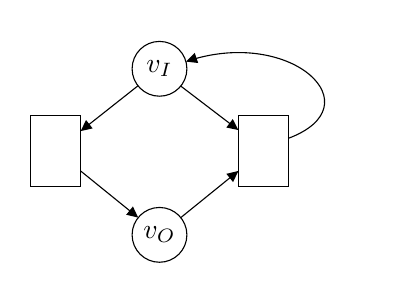
\begin{tikzpicture}[x=0.75pt,y=0.75pt,yscale=-1,xscale=1]
%uncomment if require: \path (0,200); %set diagram left start at 0, and has height of 200

%Straight Lines [id:da5988806727183245]
\draw    (120,76) -- (155.62,103.18) ;
\draw [shift={(158,105)}, rotate = 217.35] [fill={rgb, 255:red, 0; green, 0; blue, 0 }  ][line width=0.08]  [draw opacity=0] (5.36,-2.57) -- (0,0) -- (5.36,2.57) -- cycle    ;

% Text Node
\draw  [fill={rgb, 255:red, 255; green, 255; blue, 255 }  ,fill opacity=1 ]  (58,98) -- (82,98) -- (82,132) -- (58,132) -- cycle  ;
\draw (70,115) node   [align=left] {\begin{minipage}[lt]{13.600000000000001pt}\setlength\topsep{0pt}
\begin{center}
\end{center}

\end{minipage}};
% Text Node
\draw  [fill={rgb, 255:red, 255; green, 255; blue, 255 }  ,fill opacity=1 ]  (120, 75.5) circle [x radius= 13.2, y radius= 13.2]   ;
\draw (120,75.5) node   [align=left] {\begin{minipage}[lt]{14.96pt}\setlength\topsep{0pt}
\begin{center}
$\displaystyle v_{I}$
\end{center}

\end{minipage}};
% Text Node
\draw  [fill={rgb, 255:red, 255; green, 255; blue, 255 }  ,fill opacity=1 ]  (158,98) -- (182,98) -- (182,132) -- (158,132) -- cycle  ;
\draw (170,115) node   [align=left] {\begin{minipage}[lt]{13.600000000000001pt}\setlength\topsep{0pt}
\begin{center}
\end{center}

\end{minipage}};
% Text Node
\draw  [fill={rgb, 255:red, 255; green, 255; blue, 255 }  ,fill opacity=1 ]  (120, 155.5) circle [x radius= 13.2, y radius= 13.2]   ;
\draw (120,155.5) node   [align=left] {\begin{minipage}[lt]{14.96pt}\setlength\topsep{0pt}
\begin{center}
$\displaystyle v_{O}$
\end{center}

\end{minipage}};
% Connection
\draw    (109.64,83.68) -- (84.35,103.66) ;
\draw [shift={(82,105.52)}, rotate = 321.69] [fill={rgb, 255:red, 0; green, 0; blue, 0 }  ][line width=0.08]  [draw opacity=0] (5.36,-2.57) -- (0,0) -- (5.36,2.57) -- cycle    ;
% Connection
\draw    (82,124.72) -- (107.41,145.3) ;
\draw [shift={(109.74,147.19)}, rotate = 219.01] [fill={rgb, 255:red, 0; green, 0; blue, 0 }  ][line width=0.08]  [draw opacity=0] (5.36,-2.57) -- (0,0) -- (5.36,2.57) -- cycle    ;
% Connection
\draw    (130.26,147.19) -- (155.67,126.61) ;
\draw [shift={(158,124.72)}, rotate = 500.99] [fill={rgb, 255:red, 0; green, 0; blue, 0 }  ][line width=0.08]  [draw opacity=0] (5.36,-2.57) -- (0,0) -- (5.36,2.57) -- cycle    ;
% Connection
\draw    (182,109.03) .. controls (223.8,93.44) and (184.07,55.95) .. (134.99,71.28) ;
\draw [shift={(132.74,72.02)}, rotate = 341.03] [fill={rgb, 255:red, 0; green, 0; blue, 0 }  ][line width=0.08]  [draw opacity=0] (5.36,-2.57) -- (0,0) -- (5.36,2.57) -- cycle    ;

\end{tikzpicture}}
        \caption{$\mathsf{I}=\mathsf{B},\, \mathsf{O}=\mathsf{A}$}\label{subfig:subgraph1}
    \end{subfigure}
    %
    \begin{subfigure}[b]{0.3\linewidth}
        \centering
        \resizebox{.9\textwidth}{!}{

\tikzset{every picture/.style={line width=0.75pt}} %set default line width to 0.75pt

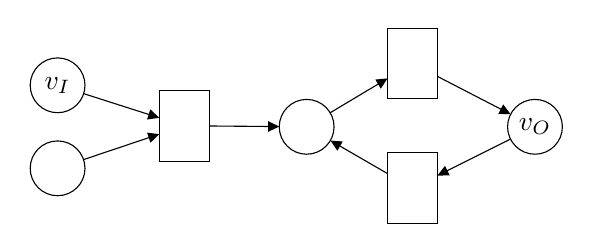
\begin{tikzpicture}[x=0.75pt,y=0.75pt,yscale=-1,xscale=1]
%uncomment if require: \path (0,128); %set diagram left start at 0, and has height of 128


% Text Node
\draw  [fill={rgb, 255:red, 255; green, 255; blue, 255 }  ,fill opacity=1 ]  (29, 41) circle [x radius= 13.2, y radius= 13.2]   ;
\draw (29,41) node   [align=left] {\begin{minipage}[lt]{14.96pt}\setlength\topsep{0pt}
\begin{center}
$\displaystyle v_{I}$
\end{center}

\end{minipage}};
% Text Node
\draw  [fill={rgb, 255:red, 255; green, 255; blue, 255 }  ,fill opacity=1 ]  (29, 81) circle [x radius= 13.2, y radius= 13.2]   ;
\draw (29,81) node   [align=left] {\begin{minipage}[lt]{14.96pt}\setlength\topsep{0pt}
\begin{center}
\end{center}

\end{minipage}};
% Text Node
\draw  [fill={rgb, 255:red, 255; green, 255; blue, 255 }  ,fill opacity=1 ]  (78,43.5) -- (102,43.5) -- (102,77.5) -- (78,77.5) -- cycle  ;
\draw (90,60.5) node   [align=left] {\begin{minipage}[lt]{13.600000000000001pt}\setlength\topsep{0pt}
\begin{center}
\end{center}

\end{minipage}};
% Text Node
\draw  [fill={rgb, 255:red, 255; green, 255; blue, 255 }  ,fill opacity=1 ]  (149, 61) circle [x radius= 13.2, y radius= 13.2]   ;
\draw (149,61) node   [align=left] {\begin{minipage}[lt]{14.96pt}\setlength\topsep{0pt}
\begin{center}
\end{center}

\end{minipage}};
% Text Node
\draw  [fill={rgb, 255:red, 255; green, 255; blue, 255 }  ,fill opacity=1 ]  (188,13.5) -- (212,13.5) -- (212,47.5) -- (188,47.5) -- cycle  ;
\draw (200,30.5) node   [align=left] {\begin{minipage}[lt]{13.600000000000001pt}\setlength\topsep{0pt}
\begin{center}
\end{center}

\end{minipage}};
% Text Node
\draw  [fill={rgb, 255:red, 255; green, 255; blue, 255 }  ,fill opacity=1 ]  (188,73.5) -- (212,73.5) -- (212,107.5) -- (188,107.5) -- cycle  ;
\draw (200,90.5) node   [align=left] {\begin{minipage}[lt]{13.600000000000001pt}\setlength\topsep{0pt}
\begin{center}
\end{center}

\end{minipage}};
% Text Node
\draw  [fill={rgb, 255:red, 255; green, 255; blue, 255 }  ,fill opacity=1 ]  (259, 61) circle [x radius= 13.2, y radius= 13.2]   ;
\draw (259,61) node   [align=left] {\begin{minipage}[lt]{14.96pt}\setlength\topsep{0pt}
\begin{center}
$\displaystyle v_{O}$
\end{center}

\end{minipage}};
% Connection
\draw    (41.58,45.02) -- (75.14,55.75) ;
\draw [shift={(78,56.66)}, rotate = 197.73] [fill={rgb, 255:red, 0; green, 0; blue, 0 }  ][line width=0.08]  [draw opacity=0] (5.36,-2.57) -- (0,0) -- (5.36,2.57) -- cycle    ;
% Connection
\draw    (41.52,76.79) -- (75.16,65.49) ;
\draw [shift={(78,64.53)}, rotate = 521.4200000000001] [fill={rgb, 255:red, 0; green, 0; blue, 0 }  ][line width=0.08]  [draw opacity=0] (5.36,-2.57) -- (0,0) -- (5.36,2.57) -- cycle    ;
% Connection
\draw    (102,60.6) -- (132.8,60.86) ;
\draw [shift={(135.8,60.89)}, rotate = 180.49] [fill={rgb, 255:red, 0; green, 0; blue, 0 }  ][line width=0.08]  [draw opacity=0] (5.36,-2.57) -- (0,0) -- (5.36,2.57) -- cycle    ;
% Connection
\draw    (160.33,54.22) -- (185.43,39.22) ;
\draw [shift={(188,37.68)}, rotate = 509.12] [fill={rgb, 255:red, 0; green, 0; blue, 0 }  ][line width=0.08]  [draw opacity=0] (5.36,-2.57) -- (0,0) -- (5.36,2.57) -- cycle    ;
% Connection
\draw    (212,36.7) -- (244.61,53.56) ;
\draw [shift={(247.27,54.94)}, rotate = 207.34] [fill={rgb, 255:red, 0; green, 0; blue, 0 }  ][line width=0.08]  [draw opacity=0] (5.36,-2.57) -- (0,0) -- (5.36,2.57) -- cycle    ;
% Connection
\draw    (247.19,66.9) -- (214.68,83.16) ;
\draw [shift={(212,84.5)}, rotate = 333.43] [fill={rgb, 255:red, 0; green, 0; blue, 0 }  ][line width=0.08]  [draw opacity=0] (5.36,-2.57) -- (0,0) -- (5.36,2.57) -- cycle    ;
% Connection
\draw    (188,83.56) -- (163.03,69.11) ;
\draw [shift={(160.43,67.61)}, rotate = 390.05] [fill={rgb, 255:red, 0; green, 0; blue, 0 }  ][line width=0.08]  [draw opacity=0] (5.36,-2.57) -- (0,0) -- (5.36,2.57) -- cycle    ;

\end{tikzpicture}}
        \caption{$\mathsf{I}=\mathsf{C},\, \mathsf{O}=\mathsf{F}$}\label{subfig:subgraph2}
    \end{subfigure}
    %
    \begin{subfigure}[b]{0.45\linewidth}
        \centering
        \resizebox{.9\textwidth}{!}{

\tikzset{every picture/.style={line width=0.75pt}} %set default line width to 0.75pt        

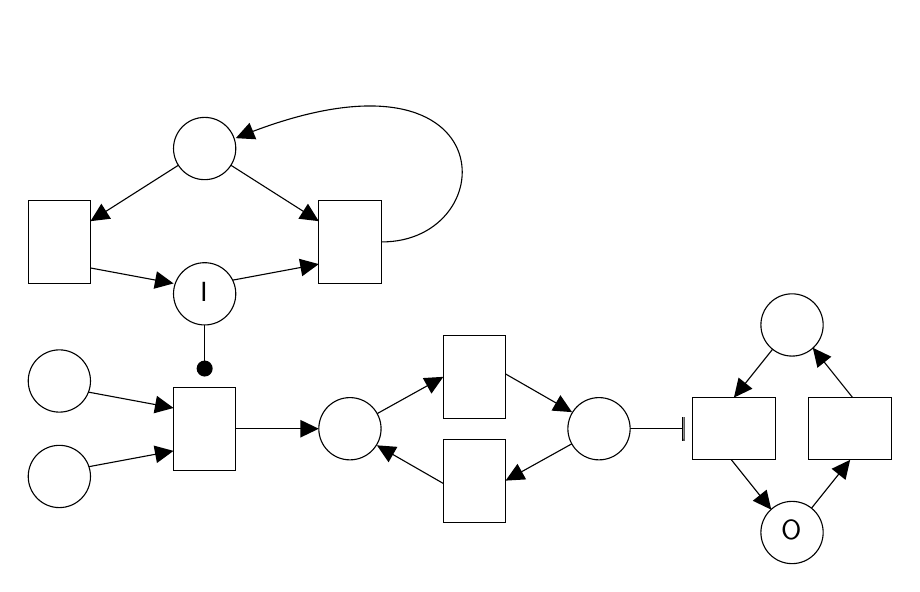
\begin{tikzpicture}[x=0.75pt,y=0.75pt,yscale=-1,xscale=1]
%uncomment if require: \path (0,263); %set diagram left start at 0, and has height of 263

%Straight Lines [id:da9076248721928286] 
\draw    (408,230) -- (434.13,197.34) ;
\draw [shift={(436,195)}, rotate = 488.66] [fill={rgb, 255:red, 0; green, 0; blue, 0 }  ][line width=0.08]  [draw opacity=0] (8.93,-4.29) -- (0,0) -- (8.93,4.29) -- cycle    ;
%Straight Lines [id:da8310282669133191] 
\draw    (370,184) -- (396.13,216.66) ;
\draw [shift={(398,219)}, rotate = 231.34] [fill={rgb, 255:red, 0; green, 0; blue, 0 }  ][line width=0.08]  [draw opacity=0] (8.93,-4.29) -- (0,0) -- (8.93,4.29) -- cycle    ;
%Straight Lines [id:da21056116046945594] 
\draw    (408,130) -- (381.87,162.66) ;
\draw [shift={(380,165)}, rotate = 308.65999999999997] [fill={rgb, 255:red, 0; green, 0; blue, 0 }  ][line width=0.08]  [draw opacity=0] (8.93,-4.29) -- (0,0) -- (8.93,4.29) -- cycle    ;
%Straight Lines [id:da5752373273055789] 
\draw    (446,176) -- (419.87,143.34) ;
\draw [shift={(418,141)}, rotate = 411.34000000000003] [fill={rgb, 255:red, 0; green, 0; blue, 0 }  ][line width=0.08]  [draw opacity=0] (8.93,-4.29) -- (0,0) -- (8.93,4.29) -- cycle    ;
%Straight Lines [id:da16579110027769128] 
\draw    (315,180) -- (355,180) ;
%Straight Lines [id:da4838109924037106] 
\draw    (130,180) -- (177,180) ;
\draw [shift={(180,180)}, rotate = 180] [fill={rgb, 255:red, 0; green, 0; blue, 0 }  ][line width=0.08]  [draw opacity=0] (8.93,-4.29) -- (0,0) -- (8.93,4.29) -- cycle    ;
%Straight Lines [id:da1725280869298207] 
\draw    (255,145) -- (299.4,170.51) ;
\draw [shift={(302,172)}, rotate = 209.88] [fill={rgb, 255:red, 0; green, 0; blue, 0 }  ][line width=0.08]  [draw opacity=0] (8.93,-4.29) -- (0,0) -- (8.93,4.29) -- cycle    ;
%Straight Lines [id:da34654117341962776] 
\draw    (255,215) -- (210.6,189.49) ;
\draw [shift={(208,188)}, rotate = 389.88] [fill={rgb, 255:red, 0; green, 0; blue, 0 }  ][line width=0.08]  [draw opacity=0] (8.93,-4.29) -- (0,0) -- (8.93,4.29) -- cycle    ;
%Straight Lines [id:da2572335252881772] 
\draw    (315,180) -- (272.62,203.54) ;
\draw [shift={(270,205)}, rotate = 330.95] [fill={rgb, 255:red, 0; green, 0; blue, 0 }  ][line width=0.08]  [draw opacity=0] (8.93,-4.29) -- (0,0) -- (8.93,4.29) -- cycle    ;
%Straight Lines [id:da9569901142124524] 
\draw    (195,180) -- (237.38,156.46) ;
\draw [shift={(240,155)}, rotate = 510.95] [fill={rgb, 255:red, 0; green, 0; blue, 0 }  ][line width=0.08]  [draw opacity=0] (8.93,-4.29) -- (0,0) -- (8.93,4.29) -- cycle    ;
%Straight Lines [id:da920112653947581] 
\draw    (130,110) -- (177.05,101.23) ;
\draw [shift={(180,100.68)}, rotate = 529.44] [fill={rgb, 255:red, 0; green, 0; blue, 0 }  ][line width=0.08]  [draw opacity=0] (8.93,-4.29) -- (0,0) -- (8.93,4.29) -- cycle    ;
%Straight Lines [id:da7419253152894756] 
\draw    (60,100.68) -- (107.05,109.45) ;
\draw [shift={(110,110)}, rotate = 190.56] [fill={rgb, 255:red, 0; green, 0; blue, 0 }  ][line width=0.08]  [draw opacity=0] (8.93,-4.29) -- (0,0) -- (8.93,4.29) -- cycle    ;
%Straight Lines [id:da9584629103768068] 
\draw    (125,45) -- (177.47,78.39) ;
\draw [shift={(180,80)}, rotate = 212.47] [fill={rgb, 255:red, 0; green, 0; blue, 0 }  ][line width=0.08]  [draw opacity=0] (8.93,-4.29) -- (0,0) -- (8.93,4.29) -- cycle    ;
%Shape: Rectangle [id:dp7470169028080813] 
\draw  [fill={rgb, 255:red, 255; green, 255; blue, 255 }  ,fill opacity=1 ] (40,70) -- (70,70) -- (70,110) -- (40,110) -- cycle ;
%Straight Lines [id:da7129571423389669] 
\draw    (125,45) -- (72.53,78.39) ;
\draw [shift={(70,80)}, rotate = 327.53] [fill={rgb, 255:red, 0; green, 0; blue, 0 }  ][line width=0.08]  [draw opacity=0] (8.93,-4.29) -- (0,0) -- (8.93,4.29) -- cycle    ;
%Shape: Circle [id:dp7911048844652653] 
\draw  [fill={rgb, 255:red, 255; green, 255; blue, 255 }  ,fill opacity=1 ] (110,45) .. controls (110,36.72) and (116.72,30) .. (125,30) .. controls (133.28,30) and (140,36.72) .. (140,45) .. controls (140,53.28) and (133.28,60) .. (125,60) .. controls (116.72,60) and (110,53.28) .. (110,45) -- cycle ;
%Shape: Rectangle [id:dp7683065667775133] 
\draw  [fill={rgb, 255:red, 255; green, 255; blue, 255 }  ,fill opacity=1 ] (180,70) -- (210,70) -- (210,110) -- (180,110) -- cycle ;
%Curve Lines [id:da44464433303214457] 
\draw    (210,90) .. controls (270.06,90.4) and (270.75,-12.96) .. (141.95,39.2) ;
\draw [shift={(140,40)}, rotate = 337.56] [fill={rgb, 255:red, 0; green, 0; blue, 0 }  ][line width=0.08]  [draw opacity=0] (8.93,-4.29) -- (0,0) -- (8.93,4.29) -- cycle    ;
%Shape: Circle [id:dp6369849547820912] 
\draw  [fill={rgb, 255:red, 255; green, 255; blue, 255 }  ,fill opacity=1 ] (110,115) .. controls (110,106.72) and (116.72,100) .. (125,100) .. controls (133.28,100) and (140,106.72) .. (140,115) .. controls (140,123.28) and (133.28,130) .. (125,130) .. controls (116.72,130) and (110,123.28) .. (110,115) -- cycle ;
%Straight Lines [id:da8558653638989671] 
\draw    (125,130) -- (125,151) ;
\draw [shift={(125,151)}, rotate = 90] [color={rgb, 255:red, 0; green, 0; blue, 0 }  ][fill={rgb, 255:red, 0; green, 0; blue, 0 }  ][line width=0.75]      (0, 0) circle [x radius= 3.35, y radius= 3.35]   ;
%Shape: Rectangle [id:dp2555616169207473] 
\draw  [fill={rgb, 255:red, 255; green, 255; blue, 255 }  ,fill opacity=1 ] (110,160) -- (140,160) -- (140,200) -- (110,200) -- cycle ;
%Straight Lines [id:da025173975162050777] 
\draw    (60,160.68) -- (107.05,169.45) ;
\draw [shift={(110,170)}, rotate = 190.56] [fill={rgb, 255:red, 0; green, 0; blue, 0 }  ][line width=0.08]  [draw opacity=0] (8.93,-4.29) -- (0,0) -- (8.93,4.29) -- cycle    ;
%Straight Lines [id:da2606365706970364] 
\draw    (60,200) -- (107.05,191.23) ;
\draw [shift={(110,190.68)}, rotate = 529.44] [fill={rgb, 255:red, 0; green, 0; blue, 0 }  ][line width=0.08]  [draw opacity=0] (8.93,-4.29) -- (0,0) -- (8.93,4.29) -- cycle    ;
%Shape: Circle [id:dp04449919596066709] 
\draw  [fill={rgb, 255:red, 255; green, 255; blue, 255 }  ,fill opacity=1 ] (40,157) .. controls (40,148.72) and (46.72,142) .. (55,142) .. controls (63.28,142) and (70,148.72) .. (70,157) .. controls (70,165.28) and (63.28,172) .. (55,172) .. controls (46.72,172) and (40,165.28) .. (40,157) -- cycle ;
%Shape: Circle [id:dp22634666421190697] 
\draw  [fill={rgb, 255:red, 255; green, 255; blue, 255 }  ,fill opacity=1 ] (40,203) .. controls (40,194.72) and (46.72,188) .. (55,188) .. controls (63.28,188) and (70,194.72) .. (70,203) .. controls (70,211.28) and (63.28,218) .. (55,218) .. controls (46.72,218) and (40,211.28) .. (40,203) -- cycle ;
%Shape: Circle [id:dp8370082251852078] 
\draw  [fill={rgb, 255:red, 255; green, 255; blue, 255 }  ,fill opacity=1 ] (180,180) .. controls (180,171.72) and (186.72,165) .. (195,165) .. controls (203.28,165) and (210,171.72) .. (210,180) .. controls (210,188.28) and (203.28,195) .. (195,195) .. controls (186.72,195) and (180,188.28) .. (180,180) -- cycle ;
%Shape: Rectangle [id:dp939444556732205] 
\draw  [fill={rgb, 255:red, 255; green, 255; blue, 255 }  ,fill opacity=1 ] (240,135) -- (270,135) -- (270,175) -- (240,175) -- cycle ;
%Shape: Rectangle [id:dp6023598592965531] 
\draw  [fill={rgb, 255:red, 255; green, 255; blue, 255 }  ,fill opacity=1 ] (240,185) -- (270,185) -- (270,225) -- (240,225) -- cycle ;
%Shape: Circle [id:dp39166844545870805] 
\draw  [fill={rgb, 255:red, 255; green, 255; blue, 255 }  ,fill opacity=1 ] (300,180) .. controls (300,171.72) and (306.72,165) .. (315,165) .. controls (323.28,165) and (330,171.72) .. (330,180) .. controls (330,188.28) and (323.28,195) .. (315,195) .. controls (306.72,195) and (300,188.28) .. (300,180) -- cycle ;
%Straight Lines [id:da6302251066776063] 
\draw    (355.29,174.43) -- (355.26,185.81) ;
%Straight Lines [id:da09616421048913337] 
\draw    (356,174.43) -- (355.97,185.81) ;
%Shape: Rectangle [id:dp49358854050629763] 
\draw  [fill={rgb, 255:red, 255; green, 255; blue, 255 }  ,fill opacity=1 ] (400,165) -- (400,195) -- (360,195) -- (360,165) -- cycle ;
%Shape: Rectangle [id:dp10449510627567582] 
\draw  [fill={rgb, 255:red, 255; green, 255; blue, 255 }  ,fill opacity=1 ] (456,165) -- (456,195) -- (416,195) -- (416,165) -- cycle ;
%Shape: Circle [id:dp5901019515208137] 
\draw  [fill={rgb, 255:red, 255; green, 255; blue, 255 }  ,fill opacity=1 ] (393,130) .. controls (393,121.72) and (399.72,115) .. (408,115) .. controls (416.28,115) and (423,121.72) .. (423,130) .. controls (423,138.28) and (416.28,145) .. (408,145) .. controls (399.72,145) and (393,138.28) .. (393,130) -- cycle ;
%Shape: Circle [id:dp23856981879081252] 
\draw  [fill={rgb, 255:red, 255; green, 255; blue, 255 }  ,fill opacity=1 ] (393,230) .. controls (393,221.72) and (399.72,215) .. (408,215) .. controls (416.28,215) and (423,221.72) .. (423,230) .. controls (423,238.28) and (416.28,245) .. (408,245) .. controls (399.72,245) and (393,238.28) .. (393,230) -- cycle ;

% Text Node
\draw (121.5,108) node [anchor=north west][inner sep=0.75pt]   [align=left] {$\mathsf{I}$};
% Text Node
\draw (401.5,223) node [anchor=north west][inner sep=0.75pt]   [align=left] {$\mathsf{O}$};


\end{tikzpicture}}
        \caption{$\mathsf{I}=\mathsf{A},\, \mathsf{O}=\mathsf{H}$}\label{subfig:subgraph3}
    \end{subfigure}
    \caption{Examples of subgraphs of the pathway graph in Figure \ref{fig:pathway-graph} induced by different input/output node pairs $(\mathsf{I},\mathsf{O})$.}\label{fig:subgraphs}
\end{figure*}
The bulk of this phase consists in associating, for a given pathway graph $G$, a set of induced subgraphs:
$$\Cal{S}_G = \Set{S_{\mathsf{I},\mathsf{O}} \mid \forall (\mathsf{I},\mathsf{O}) \in \Cal{V}_{G}^{\Fun{mol}}},\; G \in \mathbb{G},$$
for every possible pair of nodes representing molecules. After repeating this processing for each pathway graph in our dataset $\mathbb{G}$, we extracted a total 44928 induced subgraphs from the original 484 pathway graphs. After this phase, our reference dataset becomes:
$$\mathbb{G}_{\Cal{S}} = \Set{\Cal{S}_G \mid G \in \mathbb{G}}.$$

\subsection{Subgraph Features}
Subsequently, we turned the induced subgraphs into attributed subgraphs by defining their set of node and edge features. Specifically, given an induced subgraph $S_{\mathsf{I},\mathsf{O}}$ and one of its nodes $v \in \Cal{V}_{S_{\mathsf{I},\mathsf{O}}}$, we define its 3-dimensional vector of node features $\Elem{x}{v} \in \Vector{x}_{S_{\mathsf{I},\mathsf{O}}}$ component by component as follows:
\begin{align*}
    \Elem{x}{v, 1} = \begin{cases}
        1  & \mathrm{if}\; v \in \Cal{V}_{G}^{\Fun{mol}}\\
        0  & \mathrm{if}\; v \in \Cal{V}_{G}^{\Fun{rx}},
    \end{cases}
    \hspace{1.5em}
    \Elem{x}{v, 2} = \begin{cases}
        1  & \mathrm{if}\; v = \mathsf{I}\\
        0  & \mathrm{otherwise},
    \end{cases}
    \hspace{1.5em}
    \Elem{x}{v, 3} = \begin{cases}
        1  & \mathrm{if}\; v = \mathsf{O}\\
        0  & \mathrm{otherwise},
    \end{cases}
\end{align*}
where the notation $\Elem{x}{v, i}$ indicates the $i$-th component of the node feature vector $\Elem{x}{v}$.
Similarly, given an edge $(u,v) \in \Cal{E}_{S(\mathsf{I},\mathsf{O})}$, we define its 3-dimensional vector of edge features $\Elem{e}{u, v} \in \Vector{e}_{S_{\mathsf{I},\mathsf{O}}}$ component by component as follows:
\begin{align*}
    \Elem{e}{u, v, 1} = \mathbb{I}[(u,v) \in \Cal{E}_{G}^{\Fun{std}}], \quad
    \Elem{e}{u, v, 2} = \mathbb{I}[(u,v) \in \Cal{E}_{G}^{\Fun{pro}}], \quad
    \Elem{e}{u, v, 3} = \mathbb{I}[(u,v) \in \Cal{E}_{G}^{\Fun{inh}}],
\end{align*}
where $\mathbb{I}$ is the indicator function, and the notation $\Elem{e}{u, v, i}$ identifies the $i$-th component of the edge feature vector $\Elem{e}{u, v}$. Figure \ref{fig:pathway-graph-features} shows the induced subgraph of Figure \ref{subfig:subgraph3} with the corresponding feature vectors in place of its nodes and edges.

\begin{figure*}[h!]
    \centering
    \resizebox{.8\textwidth}{!}{

\tikzset{every picture/.style={line width=0.75pt}} %set default line width to 0.75pt        

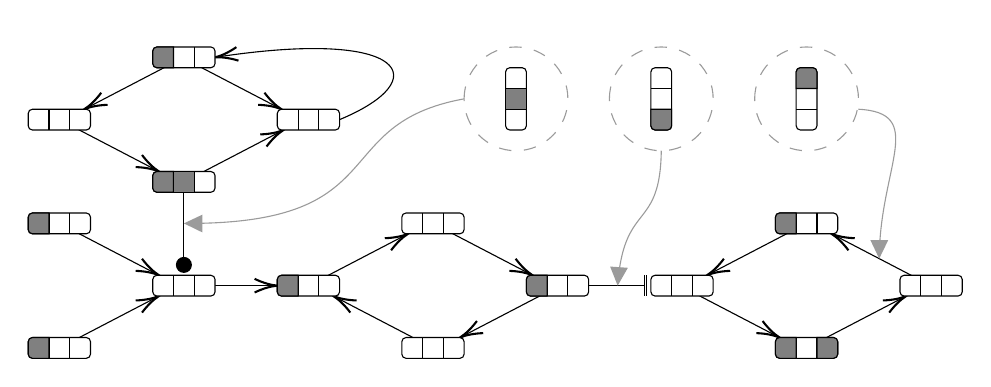
\begin{tikzpicture}[x=0.75pt,y=0.75pt,yscale=-1,xscale=1]
%uncomment if require: \path (0,300); %set diagram left start at 0, and has height of 300

%Straight Lines [id:da5482291659625731] 
\draw    (485,165) -- (438.77,140.92) ;
\draw [shift={(437,140)}, rotate = 387.51] [color={rgb, 255:red, 0; green, 0; blue, 0 }  ][line width=0.75]    (10.93,-3.29) .. controls (6.95,-1.4) and (3.31,-0.3) .. (0,0) .. controls (3.31,0.3) and (6.95,1.4) .. (10.93,3.29)   ;
%Straight Lines [id:da3558653268261338] 
\draw    (125,55) -- (78.77,79.08) ;
\draw [shift={(77,80)}, rotate = 332.49] [color={rgb, 255:red, 0; green, 0; blue, 0 }  ][line width=0.75]    (10.93,-3.29) .. controls (6.95,-1.4) and (3.31,-0.3) .. (0,0) .. controls (3.31,0.3) and (6.95,1.4) .. (10.93,3.29)   ;
%Straight Lines [id:da8145950972698188] 
\draw    (124,55) -- (170.23,79.08) ;
\draw [shift={(172,80)}, rotate = 207.51] [color={rgb, 255:red, 0; green, 0; blue, 0 }  ][line width=0.75]    (10.93,-3.29) .. controls (6.95,-1.4) and (3.31,-0.3) .. (0,0) .. controls (3.31,0.3) and (6.95,1.4) .. (10.93,3.29)   ;
%Curve Lines [id:da32133946156304494] 
\draw    (200,85) .. controls (246.69,65.62) and (232.66,40.97) .. (141.38,54.79) ;
\draw [shift={(140,55)}, rotate = 351.23] [color={rgb, 255:red, 0; green, 0; blue, 0 }  ][line width=0.75]    (10.93,-3.29) .. controls (6.95,-1.4) and (3.31,-0.3) .. (0,0) .. controls (3.31,0.3) and (6.95,1.4) .. (10.93,3.29)   ;
%Straight Lines [id:da041273036913917815] 
\draw    (65,85) -- (111.23,109.08) ;
\draw [shift={(113,110)}, rotate = 207.51] [color={rgb, 255:red, 0; green, 0; blue, 0 }  ][line width=0.75]    (10.93,-3.29) .. controls (6.95,-1.4) and (3.31,-0.3) .. (0,0) .. controls (3.31,0.3) and (6.95,1.4) .. (10.93,3.29)   ;
%Straight Lines [id:da8146569411368974] 
\draw    (125,115) -- (171.23,90.92) ;
\draw [shift={(173,90)}, rotate = 512.49] [color={rgb, 255:red, 0; green, 0; blue, 0 }  ][line width=0.75]    (10.93,-3.29) .. controls (6.95,-1.4) and (3.31,-0.3) .. (0,0) .. controls (3.31,0.3) and (6.95,1.4) .. (10.93,3.29)   ;
%Straight Lines [id:da3865035702712529] 
\draw    (125,115) -- (125,155) ;
\draw [shift={(125,155)}, rotate = 90] [color={rgb, 255:red, 0; green, 0; blue, 0 }  ][fill={rgb, 255:red, 0; green, 0; blue, 0 }  ][line width=0.75]      (0, 0) circle [x radius= 3.35, y radius= 3.35]   ;
%Straight Lines [id:da4717469304122126] 
\draw    (65,135) -- (111.23,159.08) ;
\draw [shift={(113,160)}, rotate = 207.51] [color={rgb, 255:red, 0; green, 0; blue, 0 }  ][line width=0.75]    (10.93,-3.29) .. controls (6.95,-1.4) and (3.31,-0.3) .. (0,0) .. controls (3.31,0.3) and (6.95,1.4) .. (10.93,3.29)   ;
%Straight Lines [id:da4798120333163296] 
\draw    (65,195) -- (111.23,170.92) ;
\draw [shift={(113,170)}, rotate = 512.49] [color={rgb, 255:red, 0; green, 0; blue, 0 }  ][line width=0.75]    (10.93,-3.29) .. controls (6.95,-1.4) and (3.31,-0.3) .. (0,0) .. controls (3.31,0.3) and (6.95,1.4) .. (10.93,3.29)   ;
%Straight Lines [id:da1936073846930204] 
\draw    (125,165) -- (168,165) ;
\draw [shift={(170,165)}, rotate = 180] [color={rgb, 255:red, 0; green, 0; blue, 0 }  ][line width=0.75]    (10.93,-3.29) .. controls (6.95,-1.4) and (3.31,-0.3) .. (0,0) .. controls (3.31,0.3) and (6.95,1.4) .. (10.93,3.29)   ;
%Straight Lines [id:da3160956298558728] 
\draw    (185,165) -- (231.23,140.92) ;
\draw [shift={(233,140)}, rotate = 512.49] [color={rgb, 255:red, 0; green, 0; blue, 0 }  ][line width=0.75]    (10.93,-3.29) .. controls (6.95,-1.4) and (3.31,-0.3) .. (0,0) .. controls (3.31,0.3) and (6.95,1.4) .. (10.93,3.29)   ;
%Straight Lines [id:da7125824842249591] 
\draw    (245,195) -- (198.77,170.92) ;
\draw [shift={(197,170)}, rotate = 387.51] [color={rgb, 255:red, 0; green, 0; blue, 0 }  ][line width=0.75]    (10.93,-3.29) .. controls (6.95,-1.4) and (3.31,-0.3) .. (0,0) .. controls (3.31,0.3) and (6.95,1.4) .. (10.93,3.29)   ;
%Straight Lines [id:da8854866739999274] 
\draw    (245,135) -- (291.23,159.08) ;
\draw [shift={(293,160)}, rotate = 207.51] [color={rgb, 255:red, 0; green, 0; blue, 0 }  ][line width=0.75]    (10.93,-3.29) .. controls (6.95,-1.4) and (3.31,-0.3) .. (0,0) .. controls (3.31,0.3) and (6.95,1.4) .. (10.93,3.29)   ;
%Straight Lines [id:da7803086702083197] 
\draw    (306,165) -- (259.77,189.08) ;
\draw [shift={(258,190)}, rotate = 332.49] [color={rgb, 255:red, 0; green, 0; blue, 0 }  ][line width=0.75]    (10.93,-3.29) .. controls (6.95,-1.4) and (3.31,-0.3) .. (0,0) .. controls (3.31,0.3) and (6.95,1.4) .. (10.93,3.29)   ;
%Straight Lines [id:da12899164332476598] 
\draw    (305,165) -- (347,165) ;
%Straight Lines [id:da7198750206752396] 
\draw    (425,135) -- (378.77,159.08) ;
\draw [shift={(377,160)}, rotate = 332.49] [color={rgb, 255:red, 0; green, 0; blue, 0 }  ][line width=0.75]    (10.93,-3.29) .. controls (6.95,-1.4) and (3.31,-0.3) .. (0,0) .. controls (3.31,0.3) and (6.95,1.4) .. (10.93,3.29)   ;
%Straight Lines [id:da9791465068682561] 
\draw    (364,165) -- (410.23,189.08) ;
\draw [shift={(412,190)}, rotate = 207.51] [color={rgb, 255:red, 0; green, 0; blue, 0 }  ][line width=0.75]    (10.93,-3.29) .. controls (6.95,-1.4) and (3.31,-0.3) .. (0,0) .. controls (3.31,0.3) and (6.95,1.4) .. (10.93,3.29)   ;
%Straight Lines [id:da6188188450953276] 
\draw    (425,195) -- (471.23,170.92) ;
\draw [shift={(473,170)}, rotate = 512.49] [color={rgb, 255:red, 0; green, 0; blue, 0 }  ][line width=0.75]    (10.93,-3.29) .. controls (6.95,-1.4) and (3.31,-0.3) .. (0,0) .. controls (3.31,0.3) and (6.95,1.4) .. (10.93,3.29)   ;
%Rounded Rect [id:dp8474040727349201] 
\draw  [fill={rgb, 255:red, 255; green, 255; blue, 255 }  ,fill opacity=1 ] (50,82) .. controls (50,80.9) and (50.9,80) .. (52,80) -- (78,80) .. controls (79.1,80) and (80,80.9) .. (80,82) -- (80,88) .. controls (80,89.1) and (79.1,90) .. (78,90) -- (52,90) .. controls (50.9,90) and (50,89.1) .. (50,88) -- cycle ;
%Straight Lines [id:da009868227811821173] 
\draw [fill={rgb, 255:red, 255; green, 255; blue, 255 }  ,fill opacity=1 ]   (60,80) -- (60,90) ;
%Straight Lines [id:da5531588010244222] 
\draw [fill={rgb, 255:red, 255; green, 255; blue, 255 }  ,fill opacity=1 ]   (70,80) -- (70,90) ;

%Rounded Rect [id:dp051842740859017855] 
\draw  [fill={rgb, 255:red, 255; green, 255; blue, 255 }  ,fill opacity=1 ] (110,52) .. controls (110,50.9) and (110.9,50) .. (112,50) -- (138,50) .. controls (139.1,50) and (140,50.9) .. (140,52) -- (140,58) .. controls (140,59.1) and (139.1,60) .. (138,60) -- (112,60) .. controls (110.9,60) and (110,59.1) .. (110,58) -- cycle ;
%Straight Lines [id:da9057225391135502] 
\draw [fill={rgb, 255:red, 255; green, 255; blue, 255 }  ,fill opacity=1 ]   (120,50) -- (120,60) ;
%Straight Lines [id:da6644491257645591] 
\draw [fill={rgb, 255:red, 255; green, 255; blue, 255 }  ,fill opacity=1 ]   (130,50) -- (130,60) ;

%Rounded Rect [id:dp6566561531995281] 
\draw  [fill={rgb, 255:red, 255; green, 255; blue, 255 }  ,fill opacity=1 ] (170,82) .. controls (170,80.9) and (170.9,80) .. (172,80) -- (198,80) .. controls (199.1,80) and (200,80.9) .. (200,82) -- (200,88) .. controls (200,89.1) and (199.1,90) .. (198,90) -- (172,90) .. controls (170.9,90) and (170,89.1) .. (170,88) -- cycle ;
%Straight Lines [id:da36189750423984623] 
\draw [fill={rgb, 255:red, 255; green, 255; blue, 255 }  ,fill opacity=1 ]   (180,80) -- (180,90) ;
%Straight Lines [id:da18569956496814277] 
\draw [fill={rgb, 255:red, 255; green, 255; blue, 255 }  ,fill opacity=1 ]   (190,80) -- (190,90) ;

%Rounded Rect [id:dp9774949153925689] 
\draw  [fill={rgb, 255:red, 255; green, 255; blue, 255 }  ,fill opacity=1 ] (110,112) .. controls (110,110.9) and (110.9,110) .. (112,110) -- (138,110) .. controls (139.1,110) and (140,110.9) .. (140,112) -- (140,118) .. controls (140,119.1) and (139.1,120) .. (138,120) -- (112,120) .. controls (110.9,120) and (110,119.1) .. (110,118) -- cycle ;
%Straight Lines [id:da8835613843611245] 
\draw [fill={rgb, 255:red, 255; green, 255; blue, 255 }  ,fill opacity=1 ]   (120,110) -- (120,120) ;
%Straight Lines [id:da046921024126330035] 
\draw [fill={rgb, 255:red, 255; green, 255; blue, 255 }  ,fill opacity=1 ]   (130,110) -- (130,120) ;

%Rounded Rect [id:dp9110792228160389] 
\draw  [fill={rgb, 255:red, 255; green, 255; blue, 255 }  ,fill opacity=1 ] (110,162) .. controls (110,160.9) and (110.9,160) .. (112,160) -- (138,160) .. controls (139.1,160) and (140,160.9) .. (140,162) -- (140,168) .. controls (140,169.1) and (139.1,170) .. (138,170) -- (112,170) .. controls (110.9,170) and (110,169.1) .. (110,168) -- cycle ;
%Straight Lines [id:da9579570207903243] 
\draw [fill={rgb, 255:red, 255; green, 255; blue, 255 }  ,fill opacity=1 ]   (120,160) -- (120,170) ;
%Straight Lines [id:da12487673944125555] 
\draw [fill={rgb, 255:red, 255; green, 255; blue, 255 }  ,fill opacity=1 ]   (130,160) -- (130,170) ;

%Rounded Rect [id:dp6019071628472181] 
\draw  [fill={rgb, 255:red, 255; green, 255; blue, 255 }  ,fill opacity=1 ] (50,132) .. controls (50,130.9) and (50.9,130) .. (52,130) -- (78,130) .. controls (79.1,130) and (80,130.9) .. (80,132) -- (80,138) .. controls (80,139.1) and (79.1,140) .. (78,140) -- (52,140) .. controls (50.9,140) and (50,139.1) .. (50,138) -- cycle ;
%Straight Lines [id:da07709686395947624] 
\draw [fill={rgb, 255:red, 255; green, 255; blue, 255 }  ,fill opacity=1 ]   (60,130) -- (60,140) ;
%Straight Lines [id:da4386719436852351] 
\draw [fill={rgb, 255:red, 255; green, 255; blue, 255 }  ,fill opacity=1 ]   (70,130) -- (70,140) ;

%Rounded Rect [id:dp7005531294638312] 
\draw  [fill={rgb, 255:red, 255; green, 255; blue, 255 }  ,fill opacity=1 ] (50,192) .. controls (50,190.9) and (50.9,190) .. (52,190) -- (78,190) .. controls (79.1,190) and (80,190.9) .. (80,192) -- (80,198) .. controls (80,199.1) and (79.1,200) .. (78,200) -- (52,200) .. controls (50.9,200) and (50,199.1) .. (50,198) -- cycle ;
%Straight Lines [id:da5611530770018562] 
\draw [fill={rgb, 255:red, 255; green, 255; blue, 255 }  ,fill opacity=1 ]   (60,190) -- (60,200) ;
%Straight Lines [id:da017232921254101363] 
\draw [fill={rgb, 255:red, 255; green, 255; blue, 255 }  ,fill opacity=1 ]   (70,190) -- (70,200) ;

%Rounded Rect [id:dp4827173759682435] 
\draw  [fill={rgb, 255:red, 255; green, 255; blue, 255 }  ,fill opacity=1 ] (170,162) .. controls (170,160.9) and (170.9,160) .. (172,160) -- (198,160) .. controls (199.1,160) and (200,160.9) .. (200,162) -- (200,168) .. controls (200,169.1) and (199.1,170) .. (198,170) -- (172,170) .. controls (170.9,170) and (170,169.1) .. (170,168) -- cycle ;
%Straight Lines [id:da9642172775022364] 
\draw [fill={rgb, 255:red, 255; green, 255; blue, 255 }  ,fill opacity=1 ]   (180,160) -- (180,170) ;
%Straight Lines [id:da7596136700374254] 
\draw [fill={rgb, 255:red, 255; green, 255; blue, 255 }  ,fill opacity=1 ]   (190,160) -- (190,170) ;

%Rounded Rect [id:dp6674528307093845] 
\draw  [fill={rgb, 255:red, 255; green, 255; blue, 255 }  ,fill opacity=1 ] (230,132) .. controls (230,130.9) and (230.9,130) .. (232,130) -- (258,130) .. controls (259.1,130) and (260,130.9) .. (260,132) -- (260,138) .. controls (260,139.1) and (259.1,140) .. (258,140) -- (232,140) .. controls (230.9,140) and (230,139.1) .. (230,138) -- cycle ;
%Straight Lines [id:da2821204278394096] 
\draw [fill={rgb, 255:red, 255; green, 255; blue, 255 }  ,fill opacity=1 ]   (240,130) -- (240,140) ;
%Straight Lines [id:da12264275434933958] 
\draw [fill={rgb, 255:red, 255; green, 255; blue, 255 }  ,fill opacity=1 ]   (250,130) -- (250,140) ;

%Rounded Rect [id:dp35957703897594406] 
\draw  [fill={rgb, 255:red, 255; green, 255; blue, 255 }  ,fill opacity=1 ] (290,162) .. controls (290,160.9) and (290.9,160) .. (292,160) -- (318,160) .. controls (319.1,160) and (320,160.9) .. (320,162) -- (320,168) .. controls (320,169.1) and (319.1,170) .. (318,170) -- (292,170) .. controls (290.9,170) and (290,169.1) .. (290,168) -- cycle ;
%Straight Lines [id:da523669754182625] 
\draw [fill={rgb, 255:red, 255; green, 255; blue, 255 }  ,fill opacity=1 ]   (300,160) -- (300,170) ;
%Straight Lines [id:da3829127214939474] 
\draw [fill={rgb, 255:red, 255; green, 255; blue, 255 }  ,fill opacity=1 ]   (310,160) -- (310,170) ;

%Rounded Rect [id:dp42701231482854474] 
\draw  [fill={rgb, 255:red, 255; green, 255; blue, 255 }  ,fill opacity=1 ] (230,192) .. controls (230,190.9) and (230.9,190) .. (232,190) -- (258,190) .. controls (259.1,190) and (260,190.9) .. (260,192) -- (260,198) .. controls (260,199.1) and (259.1,200) .. (258,200) -- (232,200) .. controls (230.9,200) and (230,199.1) .. (230,198) -- cycle ;
%Straight Lines [id:da42410503561121105] 
\draw [fill={rgb, 255:red, 255; green, 255; blue, 255 }  ,fill opacity=1 ]   (240,190) -- (240,200) ;
%Straight Lines [id:da3684047905504595] 
\draw [fill={rgb, 255:red, 255; green, 255; blue, 255 }  ,fill opacity=1 ]   (250,190) -- (250,200) ;

%Rounded Rect [id:dp11445404510516877] 
\draw  [fill={rgb, 255:red, 255; green, 255; blue, 255 }  ,fill opacity=1 ] (350,162) .. controls (350,160.9) and (350.9,160) .. (352,160) -- (378,160) .. controls (379.1,160) and (380,160.9) .. (380,162) -- (380,168) .. controls (380,169.1) and (379.1,170) .. (378,170) -- (352,170) .. controls (350.9,170) and (350,169.1) .. (350,168) -- cycle ;
%Straight Lines [id:da43972531825515127] 
\draw [fill={rgb, 255:red, 255; green, 255; blue, 255 }  ,fill opacity=1 ]   (360,160) -- (360,170) ;
%Straight Lines [id:da5041547924292167] 
\draw [fill={rgb, 255:red, 255; green, 255; blue, 255 }  ,fill opacity=1 ]   (370,160) -- (370,170) ;

%Rounded Rect [id:dp4489618141059677] 
\draw  [fill={rgb, 255:red, 255; green, 255; blue, 255 }  ,fill opacity=1 ] (410,132) .. controls (410,130.9) and (410.9,130) .. (412,130) -- (438,130) .. controls (439.1,130) and (440,130.9) .. (440,132) -- (440,138) .. controls (440,139.1) and (439.1,140) .. (438,140) -- (412,140) .. controls (410.9,140) and (410,139.1) .. (410,138) -- cycle ;
%Straight Lines [id:da13613343685552803] 
\draw [fill={rgb, 255:red, 255; green, 255; blue, 255 }  ,fill opacity=1 ]   (420,130) -- (420,140) ;
%Straight Lines [id:da1649141879778826] 
\draw [fill={rgb, 255:red, 255; green, 255; blue, 255 }  ,fill opacity=1 ]   (430,130) -- (430,140) ;

%Rounded Rect [id:dp085382714873663] 
\draw  [fill={rgb, 255:red, 255; green, 255; blue, 255 }  ,fill opacity=1 ] (470,162) .. controls (470,160.9) and (470.9,160) .. (472,160) -- (498,160) .. controls (499.1,160) and (500,160.9) .. (500,162) -- (500,168) .. controls (500,169.1) and (499.1,170) .. (498,170) -- (472,170) .. controls (470.9,170) and (470,169.1) .. (470,168) -- cycle ;
%Straight Lines [id:da7027806909135705] 
\draw [fill={rgb, 255:red, 255; green, 255; blue, 255 }  ,fill opacity=1 ]   (480,160) -- (480,170) ;
%Straight Lines [id:da6677143633674809] 
\draw [fill={rgb, 255:red, 255; green, 255; blue, 255 }  ,fill opacity=1 ]   (490,160) -- (490,170) ;

%Rounded Rect [id:dp23601106803709837] 
\draw  [fill={rgb, 255:red, 255; green, 255; blue, 255 }  ,fill opacity=1 ] (410,192) .. controls (410,190.9) and (410.9,190) .. (412,190) -- (438,190) .. controls (439.1,190) and (440,190.9) .. (440,192) -- (440,198) .. controls (440,199.1) and (439.1,200) .. (438,200) -- (412,200) .. controls (410.9,200) and (410,199.1) .. (410,198) -- cycle ;
%Straight Lines [id:da7303797329340842] 
\draw [fill={rgb, 255:red, 255; green, 255; blue, 255 }  ,fill opacity=1 ]   (420,190) -- (420,200) ;
%Straight Lines [id:da7412443437267568] 
\draw [fill={rgb, 255:red, 255; green, 255; blue, 255 }  ,fill opacity=1 ]   (430,190) -- (430,200) ;

%Straight Lines [id:da011003964046166548] 
\draw    (347,160) -- (347,170) ;
%Straight Lines [id:da9806624892870546] 
\draw    (348,160) -- (348,170) ;

%Rounded Same Side Corner Rect [id:dp3768094591748803] 
\draw  [fill={rgb, 255:red, 128; green, 128; blue, 128 }  ,fill opacity=1 ] (112,120) .. controls (110.9,120) and (110,119.1) .. (110,118) -- (110,112) .. controls (110,110.9) and (110.9,110) .. (112,110) -- (120,110) .. controls (120,110) and (120,110) .. (120,110) -- (120,120) .. controls (120,120) and (120,120) .. (120,120) -- cycle ;
%Rounded Same Side Corner Rect [id:dp9234675571457911] 
\draw  [fill={rgb, 255:red, 128; green, 128; blue, 128 }  ,fill opacity=1 ] (52,140) .. controls (50.9,140) and (50,139.1) .. (50,138) -- (50,132) .. controls (50,130.9) and (50.9,130) .. (52,130) -- (60,130) .. controls (60,130) and (60,130) .. (60,130) -- (60,140) .. controls (60,140) and (60,140) .. (60,140) -- cycle ;
%Rounded Same Side Corner Rect [id:dp5054471322165766] 
\draw  [fill={rgb, 255:red, 128; green, 128; blue, 128 }  ,fill opacity=1 ] (52,200) .. controls (50.9,200) and (50,199.1) .. (50,198) -- (50,192) .. controls (50,190.9) and (50.9,190) .. (52,190) -- (60,190) .. controls (60,190) and (60,190) .. (60,190) -- (60,200) .. controls (60,200) and (60,200) .. (60,200) -- cycle ;
%Rounded Same Side Corner Rect [id:dp3931764941128213] 
\draw  [fill={rgb, 255:red, 128; green, 128; blue, 128 }  ,fill opacity=1 ] (112,60) .. controls (110.9,60) and (110,59.1) .. (110,58) -- (110,52) .. controls (110,50.9) and (110.9,50) .. (112,50) -- (120,50) .. controls (120,50) and (120,50) .. (120,50) -- (120,60) .. controls (120,60) and (120,60) .. (120,60) -- cycle ;
%Rounded Same Side Corner Rect [id:dp2835639273199655] 
\draw  [fill={rgb, 255:red, 128; green, 128; blue, 128 }  ,fill opacity=1 ] (172,170) .. controls (170.9,170) and (170,169.1) .. (170,168) -- (170,162) .. controls (170,160.9) and (170.9,160) .. (172,160) -- (180,160) .. controls (180,160) and (180,160) .. (180,160) -- (180,170) .. controls (180,170) and (180,170) .. (180,170) -- cycle ;
%Rounded Same Side Corner Rect [id:dp9984840474478471] 
\draw  [fill={rgb, 255:red, 128; green, 128; blue, 128 }  ,fill opacity=1 ] (292,170) .. controls (290.9,170) and (290,169.1) .. (290,168) -- (290,162) .. controls (290,160.9) and (290.9,160) .. (292,160) -- (300,160) .. controls (300,160) and (300,160) .. (300,160) -- (300,170) .. controls (300,170) and (300,170) .. (300,170) -- cycle ;
%Rounded Same Side Corner Rect [id:dp9874301673779244] 
\draw  [fill={rgb, 255:red, 128; green, 128; blue, 128 }  ,fill opacity=1 ] (412,140) .. controls (410.9,140) and (410,139.1) .. (410,138) -- (410,132) .. controls (410,130.9) and (410.9,130) .. (412,130) -- (420,130) .. controls (420,130) and (420,130) .. (420,130) -- (420,140) .. controls (420,140) and (420,140) .. (420,140) -- cycle ;
%Rounded Same Side Corner Rect [id:dp17981279327281907] 
\draw  [fill={rgb, 255:red, 128; green, 128; blue, 128 }  ,fill opacity=1 ] (412,200) .. controls (410.9,200) and (410,199.1) .. (410,198) -- (410,192) .. controls (410,190.9) and (410.9,190) .. (412,190) -- (420,190) .. controls (420,190) and (420,190) .. (420,190) -- (420,200) .. controls (420,200) and (420,200) .. (420,200) -- cycle ;
%Shape: Rectangle [id:dp9896265723760629] 
\draw  [fill={rgb, 255:red, 128; green, 128; blue, 128 }  ,fill opacity=1 ] (120,110) -- (130,110) -- (130,120) -- (120,120) -- cycle ;
%Rounded Same Side Corner Rect [id:dp6704577445807436] 
\draw  [fill={rgb, 255:red, 128; green, 128; blue, 128 }  ,fill opacity=1 ] (438,190) .. controls (439.1,190) and (440,190.9) .. (440,192) -- (440,198) .. controls (440,199.1) and (439.1,200) .. (438,200) -- (430,200) .. controls (430,200) and (430,200) .. (430,200) -- (430,190) .. controls (430,190) and (430,190) .. (430,190) -- cycle ;
%Rounded Rect [id:dp11409130649511323] 
\draw  [fill={rgb, 255:red, 255; green, 255; blue, 255 }  ,fill opacity=1 ] (288,60) .. controls (289.1,60) and (290,60.9) .. (290,62) -- (290,88) .. controls (290,89.1) and (289.1,90) .. (288,90) -- (282,90) .. controls (280.9,90) and (280,89.1) .. (280,88) -- (280,62) .. controls (280,60.9) and (280.9,60) .. (282,60) -- cycle ;
%Straight Lines [id:da8566613339394187] 
\draw [fill={rgb, 255:red, 255; green, 255; blue, 255 }  ,fill opacity=1 ]   (290,70) -- (280,70) ;
%Straight Lines [id:da6431189043654337] 
\draw [fill={rgb, 255:red, 255; green, 255; blue, 255 }  ,fill opacity=1 ]   (290,80) -- (280,80) ;

%Curve Lines [id:da9261031951036094] 
\draw [color={rgb, 255:red, 155; green, 155; blue, 155 }  ,draw opacity=1 ]   (260,75) .. controls (193.53,87.09) and (227.36,135.17) .. (126.53,135.01) ;
\draw [shift={(125,135)}, rotate = 360.36] [fill={rgb, 255:red, 155; green, 155; blue, 155 }  ,fill opacity=1 ][line width=0.08]  [draw opacity=0] (8.93,-4.29) -- (0,0) -- (8.93,4.29) -- cycle    ;
%Shape: Circle [id:dp642495337158681] 
\draw  [color={rgb, 255:red, 155; green, 155; blue, 155 }  ,draw opacity=1 ][dash pattern={on 4.5pt off 4.5pt}] (260,75) .. controls (260,61.19) and (271.19,50) .. (285,50) .. controls (298.81,50) and (310,61.19) .. (310,75) .. controls (310,88.81) and (298.81,100) .. (285,100) .. controls (271.19,100) and (260,88.81) .. (260,75) -- cycle ;
%Rounded Rect [id:dp7279380411207359] 
\draw  [fill={rgb, 255:red, 255; green, 255; blue, 255 }  ,fill opacity=1 ] (358,60) .. controls (359.1,60) and (360,60.9) .. (360,62) -- (360,88) .. controls (360,89.1) and (359.1,90) .. (358,90) -- (352,90) .. controls (350.9,90) and (350,89.1) .. (350,88) -- (350,62) .. controls (350,60.9) and (350.9,60) .. (352,60) -- cycle ;
%Straight Lines [id:da643323388211388] 
\draw [fill={rgb, 255:red, 255; green, 255; blue, 255 }  ,fill opacity=1 ]   (360,70) -- (350,70) ;
%Straight Lines [id:da9235014852609569] 
\draw [fill={rgb, 255:red, 255; green, 255; blue, 255 }  ,fill opacity=1 ]   (360,80) -- (350,80) ;

%Shape: Circle [id:dp14795654137945813] 
\draw  [color={rgb, 255:red, 155; green, 155; blue, 155 }  ,draw opacity=1 ][dash pattern={on 4.5pt off 4.5pt}] (330,75) .. controls (330,61.19) and (341.19,50) .. (355,50) .. controls (368.81,50) and (380,61.19) .. (380,75) .. controls (380,88.81) and (368.81,100) .. (355,100) .. controls (341.19,100) and (330,88.81) .. (330,75) -- cycle ;
%Curve Lines [id:da714596365164035] 
\draw [color={rgb, 255:red, 155; green, 155; blue, 155 }  ,draw opacity=1 ]   (355,100) .. controls (354.49,138.16) and (337.75,124.67) .. (334.24,162.02) ;
\draw [shift={(334,165)}, rotate = 274.01] [fill={rgb, 255:red, 155; green, 155; blue, 155 }  ,fill opacity=1 ][line width=0.08]  [draw opacity=0] (8.93,-4.29) -- (0,0) -- (8.93,4.29) -- cycle    ;
%Rounded Rect [id:dp7787064930154233] 
\draw  [fill={rgb, 255:red, 255; green, 255; blue, 255 }  ,fill opacity=1 ] (428,60) .. controls (429.1,60) and (430,60.9) .. (430,62) -- (430,88) .. controls (430,89.1) and (429.1,90) .. (428,90) -- (422,90) .. controls (420.9,90) and (420,89.1) .. (420,88) -- (420,62) .. controls (420,60.9) and (420.9,60) .. (422,60) -- cycle ;
%Straight Lines [id:da6888394852686113] 
\draw [fill={rgb, 255:red, 255; green, 255; blue, 255 }  ,fill opacity=1 ]   (430,70) -- (420,70) ;
%Straight Lines [id:da5007706839755712] 
\draw [fill={rgb, 255:red, 255; green, 255; blue, 255 }  ,fill opacity=1 ]   (430,80) -- (420,80) ;

%Shape: Circle [id:dp9185294933885089] 
\draw  [color={rgb, 255:red, 155; green, 155; blue, 155 }  ,draw opacity=1 ][dash pattern={on 4.5pt off 4.5pt}] (400,75) .. controls (400,61.19) and (411.19,50) .. (425,50) .. controls (438.81,50) and (450,61.19) .. (450,75) .. controls (450,88.81) and (438.81,100) .. (425,100) .. controls (411.19,100) and (400,88.81) .. (400,75) -- cycle ;
%Curve Lines [id:da2587793508415681] 
\draw [color={rgb, 255:red, 155; green, 155; blue, 155 }  ,draw opacity=1 ]   (450,80) .. controls (482.54,81.72) and (461.1,106.72) .. (460.04,149.37) ;
\draw [shift={(460,152)}, rotate = 270.26] [fill={rgb, 255:red, 155; green, 155; blue, 155 }  ,fill opacity=1 ][line width=0.08]  [draw opacity=0] (8.93,-4.29) -- (0,0) -- (8.93,4.29) -- cycle    ;
%Rounded Same Side Corner Rect [id:dp9448859813691737] 
\draw  [fill={rgb, 255:red, 128; green, 128; blue, 128 }  ,fill opacity=1 ] (360,88) .. controls (360,89.1) and (359.1,90) .. (358,90) -- (352,90) .. controls (350.9,90) and (350,89.1) .. (350,88) -- (350,80) .. controls (350,80) and (350,80) .. (350,80) -- (360,80) .. controls (360,80) and (360,80) .. (360,80) -- cycle ;
%Rounded Same Side Corner Rect [id:dp22917183902440952] 
\draw  [fill={rgb, 255:red, 128; green, 128; blue, 128 }  ,fill opacity=1 ] (420,62) .. controls (420,60.9) and (420.9,60) .. (422,60) -- (428,60) .. controls (429.1,60) and (430,60.9) .. (430,62) -- (430,70) .. controls (430,70) and (430,70) .. (430,70) -- (420,70) .. controls (420,70) and (420,70) .. (420,70) -- cycle ;
%Shape: Rectangle [id:dp6259213163981312] 
\draw  [fill={rgb, 255:red, 128; green, 128; blue, 128 }  ,fill opacity=1 ] (280,70) -- (290,70) -- (290,80) -- (280,80) -- cycle ;




\end{tikzpicture}}
    \caption{Attributed.}
    \label{fig:pathway-graph-features}
\end{figure*}

So far, the dataset has the following form:
$$\Set{ \mid }$$

\subsection{Concentration Robustness Computation}
The robustness values have been computed for every possible ordered pair of molecular species on every \gls{ppn}, following the relative $\alpha$-robustness approach. The dynamics of each biochemical pathway has been simulated by applying a numerical solver (the \texttt{libRoadRunner} Python library) to its ODEs representation. Reference initial concentrations of involved molecules have been obtained from the original SBML model of each pathway. Moreover, 100 simulations have been performed for each molecule of the pathway by perturbing its initial concentration in the range $[-20\%,+20\%]$. The termination of each simulation has been set to the achievement of the steady state, with a timeout of 250 simulated time units.\footnote{The concentration values obtained at the end of the simulation are considered as steady state values also in the cases in which the timeout has been reached.} For each couple of input/output molecules, we computed the width $\alpha$ of the range of concentrations reached by the output molecules by varying the input ($\alpha$-robustness). A relative robustness $\overline{\alpha}$ has then been obtained by dividing $\alpha$ by the concentration reached by the output when the initial concentration of the input is the reference one (no perturbation). Finally, a robustness value $r \in [0,1]$ to be used in the dataset has been computed by comparing $\overline{\alpha}$ (a relative representation of the output range) with $0.4$ (a relative representation of the initial input range, that is $40\%$). Formally:
\[
r = 1 - min (1,\frac{\overline{\alpha}}{0.4})
\]